% A latex document created by ipypublish
% outline: ipypublish.templates.outline_schemas/latex_outline.latex.j2
% with segments:
% - standard-standard_packages: with standard nbconvert packages
% - standard-standard_definitions: with standard nbconvert definitions
% - ipypublish-doc_article: with the main ipypublish article setup
% - ipypublish-front_pages: with the main ipypublish title and contents page setup
% - ipypublish-biblio_natbib: with the main ipypublish bibliography
% - ipypublish-contents_output: with the main ipypublish content
% - ipypublish-contents_framed_code: with the input code wrapped and framed
% - ipypublish-glossary: with the main ipypublish glossary
%
%%%%%%%%%%%% DOCCLASS

\documentclass[10pt,parskip=half,
toc=sectionentrywithdots,
bibliography=totocnumbered,
captions=tableheading,numbers=noendperiod]{scrartcl}
%\usepackage{polyglossia}
%\setmainlanguage{british}
%\DeclareTextCommandDefault{\nobreakspace}{\leavevmode\nobreak\ }
\usepackage[british]{babel}

%%%%%%%%%%%%

%%%%%%%%%%%% PACKAGES

\usepackage[T1]{fontenc} % Nicer default font (+ math font) than Computer Modern for most use cases
\usepackage{mathpazo}
\usepackage{graphicx}
\usepackage[skip=3pt]{caption}
\usepackage{adjustbox} % Used to constrain images to a maximum size
\usepackage[table]{xcolor} % Allow colors to be defined
\usepackage{enumerate} % Needed for markdown enumerations to work
\usepackage{amsmath} % Equations
\usepackage{amssymb} % Equations
\usepackage{textcomp} % defines textquotesingle
% Hack from http://tex.stackexchange.com/a/47451/13684:
\AtBeginDocument{%
    \def\PYZsq{\textquotesingle}% Upright quotes in Pygmentized code
}
\usepackage{upquote} % Upright quotes for verbatim code
\usepackage{eurosym} % defines \euro
\usepackage[mathletters]{ucs} % Extended unicode (utf-8) support
\usepackage[utf8x]{inputenc} % Allow utf-8 characters in the tex document
\usepackage{fancyvrb} % verbatim replacement that allows latex
\usepackage{grffile} % extends the file name processing of package graphics
                        % to support a larger range
% The hyperref package gives us a pdf with properly built
% internal navigation ('pdf bookmarks' for the table of contents,
% internal cross-reference links, web links for URLs, etc.)
\usepackage{hyperref}
\usepackage{longtable} % longtable support required by pandoc >1.10
\usepackage{booktabs}  % table support for pandoc > 1.12.2
\usepackage[inline]{enumitem} % IRkernel/repr support (it uses the enumerate* environment)
\usepackage[normalem]{ulem} % ulem is needed to support strikethroughs (\sout)
                            % normalem makes italics be italics, not underlines

\usepackage{translations}
\usepackage{microtype} % improves the spacing between words and letters
\usepackage{placeins} % placement of figures
% could use \usepackage[section]{placeins} but placing in subsection in command section
% Places the float at precisely the location in the LaTeX code (with H)
\usepackage{float}
\usepackage[colorinlistoftodos,obeyFinal,textwidth=.8in]{todonotes} % to mark to-dos
% number figures, tables and equations by section
% fix for new versions of texlive (see https://tex.stackexchange.com/a/425603/107738)
\let\counterwithout\relax
\let\counterwithin\relax
\usepackage{chngcntr}
% header/footer
\usepackage[footsepline=0.25pt]{scrlayer-scrpage}

% bibliography formatting
\usepackage[numbers, square, super, sort&compress]{natbib}
% hyperlink doi's
\usepackage{doi}

    % define a code float
    \usepackage{newfloat} % to define a new float types
    \DeclareFloatingEnvironment[
        fileext=frm,placement={!ht},
        within=section,name=Code]{codecell}
    \DeclareFloatingEnvironment[
        fileext=frm,placement={!ht},
        within=section,name=Text]{textcell}
    \DeclareFloatingEnvironment[
        fileext=frm,placement={!ht},
        within=section,name=Text]{errorcell}

    \usepackage{listings} % a package for wrapping code in a box
    \usepackage[framemethod=tikz]{mdframed} % to fram code

%%%%%%%%%%%%

%%%%%%%%%%%% DEFINITIONS

% Pygments definitions

\makeatletter
\def\PY@reset{\let\PY@it=\relax \let\PY@bf=\relax%
    \let\PY@ul=\relax \let\PY@tc=\relax%
    \let\PY@bc=\relax \let\PY@ff=\relax}
\def\PY@tok#1{\csname PY@tok@#1\endcsname}
\def\PY@toks#1+{\ifx\relax#1\empty\else%
    \PY@tok{#1}\expandafter\PY@toks\fi}
\def\PY@do#1{\PY@bc{\PY@tc{\PY@ul{%
    \PY@it{\PY@bf{\PY@ff{#1}}}}}}}
\def\PY#1#2{\PY@reset\PY@toks#1+\relax+\PY@do{#2}}

\@namedef{PY@tok@w}{\def\PY@tc##1{\textcolor[rgb]{0.73,0.73,0.73}{##1}}}
\@namedef{PY@tok@c}{\let\PY@it=\textit\def\PY@tc##1{\textcolor[rgb]{0.25,0.50,0.50}{##1}}}
\@namedef{PY@tok@cp}{\def\PY@tc##1{\textcolor[rgb]{0.74,0.48,0.00}{##1}}}
\@namedef{PY@tok@k}{\let\PY@bf=\textbf\def\PY@tc##1{\textcolor[rgb]{0.00,0.50,0.00}{##1}}}
\@namedef{PY@tok@kp}{\def\PY@tc##1{\textcolor[rgb]{0.00,0.50,0.00}{##1}}}
\@namedef{PY@tok@kt}{\def\PY@tc##1{\textcolor[rgb]{0.69,0.00,0.25}{##1}}}
\@namedef{PY@tok@o}{\def\PY@tc##1{\textcolor[rgb]{0.40,0.40,0.40}{##1}}}
\@namedef{PY@tok@ow}{\let\PY@bf=\textbf\def\PY@tc##1{\textcolor[rgb]{0.67,0.13,1.00}{##1}}}
\@namedef{PY@tok@nb}{\def\PY@tc##1{\textcolor[rgb]{0.00,0.50,0.00}{##1}}}
\@namedef{PY@tok@nf}{\def\PY@tc##1{\textcolor[rgb]{0.00,0.00,1.00}{##1}}}
\@namedef{PY@tok@nc}{\let\PY@bf=\textbf\def\PY@tc##1{\textcolor[rgb]{0.00,0.00,1.00}{##1}}}
\@namedef{PY@tok@nn}{\let\PY@bf=\textbf\def\PY@tc##1{\textcolor[rgb]{0.00,0.00,1.00}{##1}}}
\@namedef{PY@tok@ne}{\let\PY@bf=\textbf\def\PY@tc##1{\textcolor[rgb]{0.82,0.25,0.23}{##1}}}
\@namedef{PY@tok@nv}{\def\PY@tc##1{\textcolor[rgb]{0.10,0.09,0.49}{##1}}}
\@namedef{PY@tok@no}{\def\PY@tc##1{\textcolor[rgb]{0.53,0.00,0.00}{##1}}}
\@namedef{PY@tok@nl}{\def\PY@tc##1{\textcolor[rgb]{0.63,0.63,0.00}{##1}}}
\@namedef{PY@tok@ni}{\let\PY@bf=\textbf\def\PY@tc##1{\textcolor[rgb]{0.60,0.60,0.60}{##1}}}
\@namedef{PY@tok@na}{\def\PY@tc##1{\textcolor[rgb]{0.49,0.56,0.16}{##1}}}
\@namedef{PY@tok@nt}{\let\PY@bf=\textbf\def\PY@tc##1{\textcolor[rgb]{0.00,0.50,0.00}{##1}}}
\@namedef{PY@tok@nd}{\def\PY@tc##1{\textcolor[rgb]{0.67,0.13,1.00}{##1}}}
\@namedef{PY@tok@s}{\def\PY@tc##1{\textcolor[rgb]{0.73,0.13,0.13}{##1}}}
\@namedef{PY@tok@sd}{\let\PY@it=\textit\def\PY@tc##1{\textcolor[rgb]{0.73,0.13,0.13}{##1}}}
\@namedef{PY@tok@si}{\let\PY@bf=\textbf\def\PY@tc##1{\textcolor[rgb]{0.73,0.40,0.53}{##1}}}
\@namedef{PY@tok@se}{\let\PY@bf=\textbf\def\PY@tc##1{\textcolor[rgb]{0.73,0.40,0.13}{##1}}}
\@namedef{PY@tok@sr}{\def\PY@tc##1{\textcolor[rgb]{0.73,0.40,0.53}{##1}}}
\@namedef{PY@tok@ss}{\def\PY@tc##1{\textcolor[rgb]{0.10,0.09,0.49}{##1}}}
\@namedef{PY@tok@sx}{\def\PY@tc##1{\textcolor[rgb]{0.00,0.50,0.00}{##1}}}
\@namedef{PY@tok@m}{\def\PY@tc##1{\textcolor[rgb]{0.40,0.40,0.40}{##1}}}
\@namedef{PY@tok@gh}{\let\PY@bf=\textbf\def\PY@tc##1{\textcolor[rgb]{0.00,0.00,0.50}{##1}}}
\@namedef{PY@tok@gu}{\let\PY@bf=\textbf\def\PY@tc##1{\textcolor[rgb]{0.50,0.00,0.50}{##1}}}
\@namedef{PY@tok@gd}{\def\PY@tc##1{\textcolor[rgb]{0.63,0.00,0.00}{##1}}}
\@namedef{PY@tok@gi}{\def\PY@tc##1{\textcolor[rgb]{0.00,0.63,0.00}{##1}}}
\@namedef{PY@tok@gr}{\def\PY@tc##1{\textcolor[rgb]{1.00,0.00,0.00}{##1}}}
\@namedef{PY@tok@ge}{\let\PY@it=\textit}
\@namedef{PY@tok@gs}{\let\PY@bf=\textbf}
\@namedef{PY@tok@gp}{\let\PY@bf=\textbf\def\PY@tc##1{\textcolor[rgb]{0.00,0.00,0.50}{##1}}}
\@namedef{PY@tok@go}{\def\PY@tc##1{\textcolor[rgb]{0.53,0.53,0.53}{##1}}}
\@namedef{PY@tok@gt}{\def\PY@tc##1{\textcolor[rgb]{0.00,0.27,0.87}{##1}}}
\@namedef{PY@tok@err}{\def\PY@bc##1{{\setlength{\fboxsep}{\string -\fboxrule}\fcolorbox[rgb]{1.00,0.00,0.00}{1,1,1}{\strut ##1}}}}
\@namedef{PY@tok@kc}{\let\PY@bf=\textbf\def\PY@tc##1{\textcolor[rgb]{0.00,0.50,0.00}{##1}}}
\@namedef{PY@tok@kd}{\let\PY@bf=\textbf\def\PY@tc##1{\textcolor[rgb]{0.00,0.50,0.00}{##1}}}
\@namedef{PY@tok@kn}{\let\PY@bf=\textbf\def\PY@tc##1{\textcolor[rgb]{0.00,0.50,0.00}{##1}}}
\@namedef{PY@tok@kr}{\let\PY@bf=\textbf\def\PY@tc##1{\textcolor[rgb]{0.00,0.50,0.00}{##1}}}
\@namedef{PY@tok@bp}{\def\PY@tc##1{\textcolor[rgb]{0.00,0.50,0.00}{##1}}}
\@namedef{PY@tok@fm}{\def\PY@tc##1{\textcolor[rgb]{0.00,0.00,1.00}{##1}}}
\@namedef{PY@tok@vc}{\def\PY@tc##1{\textcolor[rgb]{0.10,0.09,0.49}{##1}}}
\@namedef{PY@tok@vg}{\def\PY@tc##1{\textcolor[rgb]{0.10,0.09,0.49}{##1}}}
\@namedef{PY@tok@vi}{\def\PY@tc##1{\textcolor[rgb]{0.10,0.09,0.49}{##1}}}
\@namedef{PY@tok@vm}{\def\PY@tc##1{\textcolor[rgb]{0.10,0.09,0.49}{##1}}}
\@namedef{PY@tok@sa}{\def\PY@tc##1{\textcolor[rgb]{0.73,0.13,0.13}{##1}}}
\@namedef{PY@tok@sb}{\def\PY@tc##1{\textcolor[rgb]{0.73,0.13,0.13}{##1}}}
\@namedef{PY@tok@sc}{\def\PY@tc##1{\textcolor[rgb]{0.73,0.13,0.13}{##1}}}
\@namedef{PY@tok@dl}{\def\PY@tc##1{\textcolor[rgb]{0.73,0.13,0.13}{##1}}}
\@namedef{PY@tok@s2}{\def\PY@tc##1{\textcolor[rgb]{0.73,0.13,0.13}{##1}}}
\@namedef{PY@tok@sh}{\def\PY@tc##1{\textcolor[rgb]{0.73,0.13,0.13}{##1}}}
\@namedef{PY@tok@s1}{\def\PY@tc##1{\textcolor[rgb]{0.73,0.13,0.13}{##1}}}
\@namedef{PY@tok@mb}{\def\PY@tc##1{\textcolor[rgb]{0.40,0.40,0.40}{##1}}}
\@namedef{PY@tok@mf}{\def\PY@tc##1{\textcolor[rgb]{0.40,0.40,0.40}{##1}}}
\@namedef{PY@tok@mh}{\def\PY@tc##1{\textcolor[rgb]{0.40,0.40,0.40}{##1}}}
\@namedef{PY@tok@mi}{\def\PY@tc##1{\textcolor[rgb]{0.40,0.40,0.40}{##1}}}
\@namedef{PY@tok@il}{\def\PY@tc##1{\textcolor[rgb]{0.40,0.40,0.40}{##1}}}
\@namedef{PY@tok@mo}{\def\PY@tc##1{\textcolor[rgb]{0.40,0.40,0.40}{##1}}}
\@namedef{PY@tok@ch}{\let\PY@it=\textit\def\PY@tc##1{\textcolor[rgb]{0.25,0.50,0.50}{##1}}}
\@namedef{PY@tok@cm}{\let\PY@it=\textit\def\PY@tc##1{\textcolor[rgb]{0.25,0.50,0.50}{##1}}}
\@namedef{PY@tok@cpf}{\let\PY@it=\textit\def\PY@tc##1{\textcolor[rgb]{0.25,0.50,0.50}{##1}}}
\@namedef{PY@tok@c1}{\let\PY@it=\textit\def\PY@tc##1{\textcolor[rgb]{0.25,0.50,0.50}{##1}}}
\@namedef{PY@tok@cs}{\let\PY@it=\textit\def\PY@tc##1{\textcolor[rgb]{0.25,0.50,0.50}{##1}}}

\def\PYZbs{\char`\\}
\def\PYZus{\char`\_}
\def\PYZob{\char`\{}
\def\PYZcb{\char`\}}
\def\PYZca{\char`\^}
\def\PYZam{\char`\&}
\def\PYZlt{\char`\<}
\def\PYZgt{\char`\>}
\def\PYZsh{\char`\#}
\def\PYZpc{\char`\%}
\def\PYZdl{\char`\$}
\def\PYZhy{\char`\-}
\def\PYZsq{\char`\'}
\def\PYZdq{\char`\"}
\def\PYZti{\char`\~}
% for compatibility with earlier versions
\def\PYZat{@}
\def\PYZlb{[}
\def\PYZrb{]}
\makeatother

% ANSI colors
\definecolor{ansi-black}{HTML}{3E424D}
\definecolor{ansi-black-intense}{HTML}{282C36}
\definecolor{ansi-red}{HTML}{E75C58}
\definecolor{ansi-red-intense}{HTML}{B22B31}
\definecolor{ansi-green}{HTML}{00A250}
\definecolor{ansi-green-intense}{HTML}{007427}
\definecolor{ansi-yellow}{HTML}{DDB62B}
\definecolor{ansi-yellow-intense}{HTML}{B27D12}
\definecolor{ansi-blue}{HTML}{208FFB}
\definecolor{ansi-blue-intense}{HTML}{0065CA}
\definecolor{ansi-magenta}{HTML}{D160C4}
\definecolor{ansi-magenta-intense}{HTML}{A03196}
\definecolor{ansi-cyan}{HTML}{60C6C8}
\definecolor{ansi-cyan-intense}{HTML}{258F8F}
\definecolor{ansi-white}{HTML}{C5C1B4}
\definecolor{ansi-white-intense}{HTML}{A1A6B2}

% commands and environments needed by pandoc snippets
% extracted from the output of `pandoc -s`
\providecommand{\tightlist}{%
  \setlength{\itemsep}{0pt}\setlength{\parskip}{0pt}}
\DefineVerbatimEnvironment{Highlighting}{Verbatim}{commandchars=\\\{\}}
% Add ',fontsize=\small' for more characters per line
\newenvironment{Shaded}{}{}
\newcommand{\KeywordTok}[1]{\textcolor[rgb]{0.00,0.44,0.13}{\textbf{{#1}}}}
\newcommand{\DataTypeTok}[1]{\textcolor[rgb]{0.56,0.13,0.00}{{#1}}}
\newcommand{\DecValTok}[1]{\textcolor[rgb]{0.25,0.63,0.44}{{#1}}}
\newcommand{\BaseNTok}[1]{\textcolor[rgb]{0.25,0.63,0.44}{{#1}}}
\newcommand{\FloatTok}[1]{\textcolor[rgb]{0.25,0.63,0.44}{{#1}}}
\newcommand{\CharTok}[1]{\textcolor[rgb]{0.25,0.44,0.63}{{#1}}}
\newcommand{\StringTok}[1]{\textcolor[rgb]{0.25,0.44,0.63}{{#1}}}
\newcommand{\CommentTok}[1]{\textcolor[rgb]{0.38,0.63,0.69}{\textit{{#1}}}}
\newcommand{\OtherTok}[1]{\textcolor[rgb]{0.00,0.44,0.13}{{#1}}}
\newcommand{\AlertTok}[1]{\textcolor[rgb]{1.00,0.00,0.00}{\textbf{{#1}}}}
\newcommand{\FunctionTok}[1]{\textcolor[rgb]{0.02,0.16,0.49}{{#1}}}
\newcommand{\RegionMarkerTok}[1]{{#1}}
\newcommand{\ErrorTok}[1]{\textcolor[rgb]{1.00,0.00,0.00}{\textbf{{#1}}}}
\newcommand{\NormalTok}[1]{{#1}}

% Additional commands for more recent versions of Pandoc
\newcommand{\ConstantTok}[1]{\textcolor[rgb]{0.53,0.00,0.00}{{#1}}}
\newcommand{\SpecialCharTok}[1]{\textcolor[rgb]{0.25,0.44,0.63}{{#1}}}
\newcommand{\VerbatimStringTok}[1]{\textcolor[rgb]{0.25,0.44,0.63}{{#1}}}
\newcommand{\SpecialStringTok}[1]{\textcolor[rgb]{0.73,0.40,0.53}{{#1}}}
\newcommand{\ImportTok}[1]{{#1}}
\newcommand{\DocumentationTok}[1]{\textcolor[rgb]{0.73,0.13,0.13}{\textit{{#1}}}}
\newcommand{\AnnotationTok}[1]{\textcolor[rgb]{0.38,0.63,0.69}{\textbf{\textit{{#1}}}}}
\newcommand{\CommentVarTok}[1]{\textcolor[rgb]{0.38,0.63,0.69}{\textbf{\textit{{#1}}}}}
\newcommand{\VariableTok}[1]{\textcolor[rgb]{0.10,0.09,0.49}{{#1}}}
\newcommand{\ControlFlowTok}[1]{\textcolor[rgb]{0.00,0.44,0.13}{\textbf{{#1}}}}
\newcommand{\OperatorTok}[1]{\textcolor[rgb]{0.40,0.40,0.40}{{#1}}}
\newcommand{\BuiltInTok}[1]{{#1}}
\newcommand{\ExtensionTok}[1]{{#1}}
\newcommand{\PreprocessorTok}[1]{\textcolor[rgb]{0.74,0.48,0.00}{{#1}}}
\newcommand{\AttributeTok}[1]{\textcolor[rgb]{0.49,0.56,0.16}{{#1}}}
\newcommand{\InformationTok}[1]{\textcolor[rgb]{0.38,0.63,0.69}{\textbf{\textit{{#1}}}}}
\newcommand{\WarningTok}[1]{\textcolor[rgb]{0.38,0.63,0.69}{\textbf{\textit{{#1}}}}}

% Define a nice break command that doesn't care if a line doesn't already
% exist.
\def\br{\hspace*{\fill} \\* }

% Math Jax compatability definitions
\def\gt{>}
\def\lt{<}

\setcounter{secnumdepth}{5}

% Colors for the hyperref package
\definecolor{urlcolor}{rgb}{0,.145,.698}
\definecolor{linkcolor}{rgb}{.71,0.21,0.01}
\definecolor{citecolor}{rgb}{.12,.54,.11}

\DeclareTranslationFallback{Author}{Author}
\DeclareTranslation{Portuges}{Author}{Autor}

\DeclareTranslationFallback{List of Codes}{List of Codes}
\DeclareTranslation{Catalan}{List of Codes}{Llista de Codis}
\DeclareTranslation{Danish}{List of Codes}{Liste over Koder}
\DeclareTranslation{German}{List of Codes}{Liste der Codes}
\DeclareTranslation{Spanish}{List of Codes}{Lista de C\'{o}digos}
\DeclareTranslation{French}{List of Codes}{Liste des Codes}
\DeclareTranslation{Italian}{List of Codes}{Elenco dei Codici}
\DeclareTranslation{Dutch}{List of Codes}{Lijst van Codes}
\DeclareTranslation{Portuges}{List of Codes}{Lista de C\'{o}digos}

\DeclareTranslationFallback{Supervisors}{Supervisors}
\DeclareTranslation{Catalan}{Supervisors}{Supervisors}
\DeclareTranslation{Danish}{Supervisors}{Vejledere}
\DeclareTranslation{German}{Supervisors}{Vorgesetzten}
\DeclareTranslation{Spanish}{Supervisors}{Supervisores}
\DeclareTranslation{French}{Supervisors}{Superviseurs}
\DeclareTranslation{Italian}{Supervisors}{Le autorit\`{a} di vigilanza}
\DeclareTranslation{Dutch}{Supervisors}{supervisors}
\DeclareTranslation{Portuguese}{Supervisors}{Supervisores}

\definecolor{codegreen}{rgb}{0,0.6,0}
\definecolor{codegray}{rgb}{0.5,0.5,0.5}
\definecolor{codepurple}{rgb}{0.58,0,0.82}
\definecolor{backcolour}{rgb}{0.95,0.95,0.95}

\lstdefinestyle{mystyle}{
    commentstyle=\color{codegreen},
    keywordstyle=\color{magenta},
    numberstyle=\tiny\color{codegray},
    stringstyle=\color{codepurple},
    basicstyle=\ttfamily,
    breakatwhitespace=false,
    keepspaces=true,
    numbers=left,
    numbersep=10pt,
    showspaces=false,
    showstringspaces=false,
    showtabs=false,
    tabsize=2,
    breaklines=true,
    literate={\-}{}{0\discretionary{-}{}{-}},
  postbreak=\mbox{\textcolor{red}{$\hookrightarrow$}\space},
}

\lstset{style=mystyle}

\surroundwithmdframed[
  hidealllines=true,
  backgroundcolor=backcolour,
  innerleftmargin=0pt,
  innerrightmargin=0pt,
  innertopmargin=0pt,
  innerbottommargin=0pt]{lstlisting}

%%%%%%%%%%%%

%%%%%%%%%%%% MARGINS

 % Used to adjust the document margins
\usepackage{geometry}
\geometry{tmargin=1in,bmargin=1in,lmargin=1in,rmargin=1in,
nohead,includefoot,footskip=25pt}
% you can use showframe option to check the margins visually
%%%%%%%%%%%%

%%%%%%%%%%%% COMMANDS

% ensure new section starts on new page
\addtokomafont{section}{\clearpage}

% Prevent overflowing lines due to hard-to-break entities
\sloppy

% Setup hyperref package
\hypersetup{
    breaklinks=true,  % so long urls are correctly broken across lines
    colorlinks=true,
    urlcolor=urlcolor,
    linkcolor=linkcolor,
    citecolor=citecolor,
    }

% ensure figures are placed within subsections
\makeatletter
\AtBeginDocument{%
    \expandafter\renewcommand\expandafter\subsection\expandafter
    {\expandafter\@fb@secFB\subsection}%
    \newcommand\@fb@secFB{\FloatBarrier
    \gdef\@fb@afterHHook{\@fb@topbarrier \gdef\@fb@afterHHook{}}}%
    \g@addto@macro\@afterheading{\@fb@afterHHook}%
    \gdef\@fb@afterHHook{}%
}
\makeatother

% number figures, tables and equations by section
\counterwithout{figure}{section}
\counterwithout{table}{section}
\counterwithout{equation}{section}
\makeatletter
\@addtoreset{table}{section}
\@addtoreset{figure}{section}
\@addtoreset{equation}{section}
\makeatother
\renewcommand\thetable{\thesection.\arabic{table}}
\renewcommand\thefigure{\thesection.\arabic{figure}}
\renewcommand\theequation{\thesection.\arabic{equation}}

    % set global options for float placement
    \makeatletter
        \providecommand*\setfloatlocations[2]{\@namedef{fps@#1}{#2}}
    \makeatother

% align captions to left (indented)
\captionsetup{justification=raggedright,
singlelinecheck=false,format=hang,labelfont={it,bf}}

% shift footer down so space between separation line
\ModifyLayer[addvoffset=.6ex]{scrheadings.foot.odd}
\ModifyLayer[addvoffset=.6ex]{scrheadings.foot.even}
\ModifyLayer[addvoffset=.6ex]{scrheadings.foot.oneside}
\ModifyLayer[addvoffset=.6ex]{plain.scrheadings.foot.odd}
\ModifyLayer[addvoffset=.6ex]{plain.scrheadings.foot.even}
\ModifyLayer[addvoffset=.6ex]{plain.scrheadings.foot.oneside}
\pagestyle{scrheadings}
\clearscrheadfoot{}
\ifoot{\leftmark}
\renewcommand{\sectionmark}[1]{\markleft{\thesection\ #1}}
\ofoot{\pagemark}
\cfoot{}

%%%%%%%%%%%%

%%%%%%%%%%%% FINAL HEADER MATERIAL

% clereref must be loaded after anything that changes the referencing system
\usepackage{cleveref}
\creflabelformat{equation}{#2#1#3}

% make the code float work with cleverref
\crefname{codecell}{code}{codes}
\Crefname{codecell}{code}{codes}
% make the text float work with cleverref
\crefname{textcell}{text}{texts}
\Crefname{textcell}{text}{texts}
% make the text float work with cleverref
\crefname{errorcell}{error}{errors}
\Crefname{errorcell}{error}{errors}

%%%%%%%%%%%%

\begin{document}

    \begin{titlepage}
  \begin{flushright}
    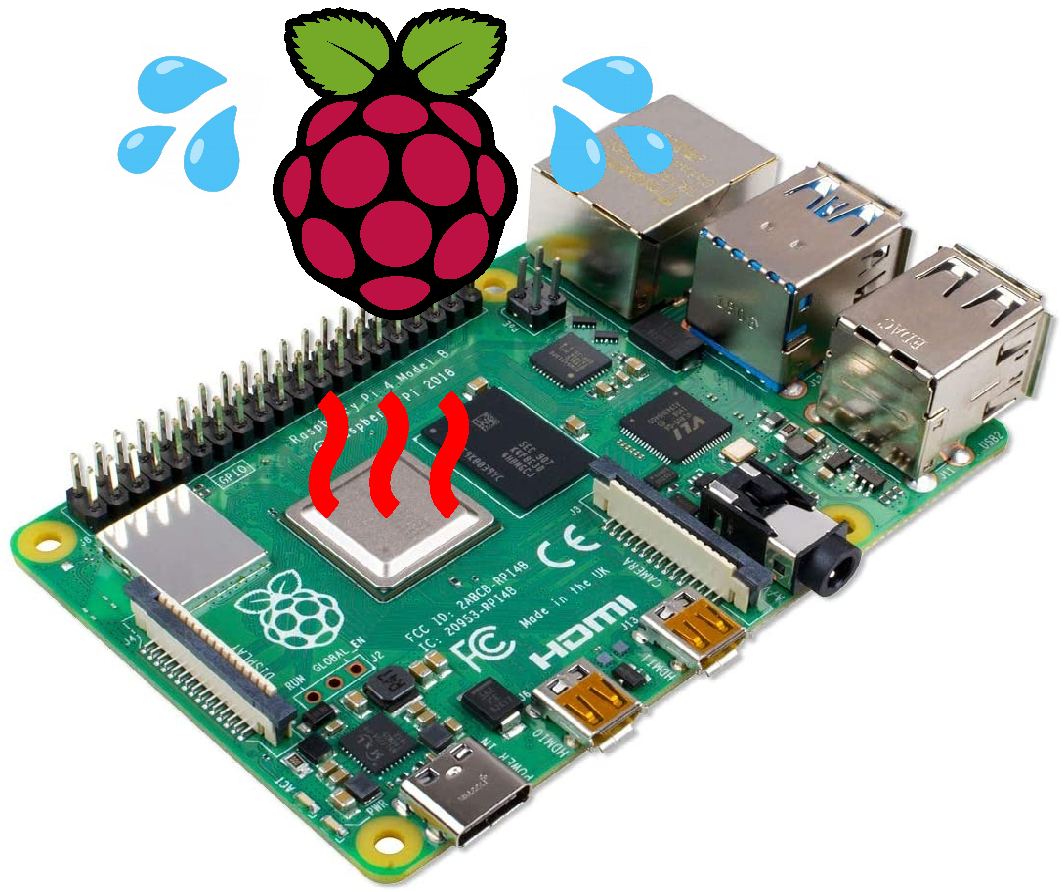
\includegraphics[width=0.7\textwidth]{Raspberry_Pi4_stress_test_files/Cover_image.pdf}
  \end{flushright}

  \begin{center}

  \vspace*{1cm}

  \Huge\textbf{Stress tests with Raspberry Pi 4 and 3B+}

  \vspace{0.5cm}

  \vspace{1.5cm}

  \begin{minipage}{0.8\textwidth}
    \begin{center}
    \begin{minipage}{0.39\textwidth}
    \begin{flushleft} \Large
    \emph{\GetTranslation{Author}:}\\Björn Kasper\\\href{mailto:bjoern.kasper@online.de}{bjoern.kasper@online.de}
    \end{flushleft}
    \end{minipage}
    \hspace{\fill}
    \begin{minipage}{0.39\textwidth}
    \begin{flushright} \Large
    \end{flushright}
    \end{minipage}
    \end{center}
  \end{minipage}

  \vfill

  \begin{minipage}{0.8\textwidth}
  \begin{center}
  \end{center}
  \end{minipage}

  \vspace{0.8cm}

  \vspace{0.4cm}

  \today

  \end{center}
  \end{titlepage}

    \begingroup
    \let\cleardoublepage\relax
    \let\clearpage\relax\tableofcontents\listoffigures\listof{codecell}{\GetTranslation{List of Codes}}
    \endgroup

\hypertarget{introduction}{%
\section{Introduction}\label{introduction}}

The aim of this notebook is to stress the Raspberry Pi 4 for deciding
between different cases and cooling types.

Sources (small selection):

\begin{itemize}
\tightlist
\item
  \url{https://github.com/nschloe/stressberry}
\item
  \url{https://www.pragmaticlinux.com/2020/06/check-the-raspberry-pi-cpu-temperature/}
\item
  \url{https://www.raspberrypi.org/blog/thermal-testing-raspberry-pi-4/}
\item
  \url{http://blog.juliusschulz.de/blog/ultimate-ipython-notebook}
\end{itemize}

\hypertarget{load-globally-used-libraries-and-set-plot-parameters}{%
\subsection{Load globally used libraries and set plot
parameters}\label{load-globally-used-libraries-and-set-plot-parameters}}

\begin{codecell}[H]
\caption{Globally used libraries and plot parameters}
\label{code:libraries_global}
\begin{lstlisting}[language=Python,numbers=left,xleftmargin=20pt,xrightmargin=5pt,belowskip=5pt,aboveskip=5pt]
import subprocess
import os
import threading
import time
import copy

#import smbus2
#import bme280

import pandas as pd
import numpy as np
#import prettytable as pt

import matplotlib.pyplot as plt
import matplotlib.dates as mdates
%matplotlib inline

# FutureWarning: Using an implicitly registered datetime converter for a matplotlib plotting method.
# The converter was registered by pandas on import.
# Future versions of pandas will require you to explicitly register matplotlib converters.
from pandas.plotting import register_matplotlib_converters
register_matplotlib_converters()

from IPython.display import set_matplotlib_formats
#matplotlib.matplotlib_inline.backend_inline.set_matplotlib_formats('pdf', 'png')
set_matplotlib_formats('pdf', 'png')

plt.rcParams['savefig.dpi'] = 80
plt.rcParams['savefig.bbox'] = "tight"

plt.rcParams['figure.autolayout'] = False
plt.rcParams['figure.figsize'] = 10, 6
plt.rcParams['axes.labelsize'] = 18
plt.rcParams['axes.titlesize'] = 20
plt.rcParams['font.size'] = 16
plt.rcParams['lines.linewidth'] = 2.0
plt.rcParams['lines.markersize'] = 8
plt.rcParams['legend.fontsize'] = 14

# Need to install dependent package first via 'apt install cm-super'
plt.rcParams['text.usetex'] = True
plt.rcParams['font.family'] = "serif"
plt.rcParams['font.serif'] = "cm"

from IPython.display import display, display_markdown, Latex
from IPython.display import Image
\end{lstlisting}\end{codecell}

\begin{lstlisting}[language={},postbreak={},numbers=none,xrightmargin=7pt,belowskip=5pt,aboveskip=5pt,breakindent=0pt]
/tmp/ipykernel_7266/1355000292.py:26: DeprecationWarning: `set_matplotlib_formats` is deprecated since IPython 7.23, directly use `matplotlib_inline.backend_inline.set_matplotlib_formats()`
  set_matplotlib_formats('pdf', 'png')

\end{lstlisting}

\hypertarget{define-all-cooling-and-ventilation-scenarios}{%
\section{Define all cooling and ventilation
scenarios}\label{define-all-cooling-and-ventilation-scenarios}}

The following cooling and ventilation scenarios are to be tested and
measured for the \textbf{Raspberry Pi B4}. For the assignment of the
experimental setups, the unique scenario IDs are in parentheses.

\hypertarget{raspberry-pi-b4-passive-cooling-without-fan}{%
\subsection{Raspberry Pi B4: Passive cooling (without
fan)}\label{raspberry-pi-b4-passive-cooling-without-fan}}

\hypertarget{without-heat-sinks}{%
\subsubsection{Without heat sinks}\label{without-heat-sinks}}

\begin{itemize}
\tightlist
\item
  with well ventilated case \textbf{\emph{(scen\_id\_01)}}
\end{itemize}

\hypertarget{with-aluminum-heat-sinks}{%
\subsubsection{With aluminum heat
sinks}\label{with-aluminum-heat-sinks}}

\begin{itemize}
\tightlist
\item
  thermal coupling: double-sided thermal tape

  \begin{itemize}
  \tightlist
  \item
    well ventilated case \textbf{\emph{(scen\_id\_02)}}
  \item
    tightly closed pink Raspberry Pi case \textbf{\emph{(scen\_id\_03)}}
  \end{itemize}
\item
  thermal coupling: silicone pads

  \begin{itemize}
  \tightlist
  \item
    well ventilated case \textbf{\emph{(scen\_id\_04)}}
  \end{itemize}
\end{itemize}

\hypertarget{with-copper-heat-sink-cpu}{%
\subsubsection{With copper heat sink
(CPU)}\label{with-copper-heat-sink-cpu}}

\begin{itemize}
\tightlist
\item
  thermal coupling: silicone pad

  \begin{itemize}
  \tightlist
  \item
    well ventilated case \textbf{\emph{(scen\_id\_05)}}
  \end{itemize}
\end{itemize}

\hypertarget{raspberry-pi-b4-active-cooling-with-fan}{%
\subsection{Raspberry Pi B4: Active cooling (with
fan)}\label{raspberry-pi-b4-active-cooling-with-fan}}

\hypertarget{with-aluminum-heat-sinks}{%
\subsubsection{With aluminum heat
sinks}\label{with-aluminum-heat-sinks}}

\begin{itemize}
\tightlist
\item
  thermal coupling: double-sided thermal tape in well-ventilated case

  \begin{itemize}
  \tightlist
  \item
    with cheap, noisy fan

    \begin{itemize}
    \tightlist
    \item
      fast speed via 5 V connection

      \begin{itemize}
      \tightlist
      \item
        blowing onto heat sink \textbf{\emph{(scen\_id\_06)}}
      \item
        blowing away from heat sink \textbf{\emph{(scen\_id\_07)}}
      \end{itemize}
    \item
      slow speed via 3.3 V connection

      \begin{itemize}
      \tightlist
      \item
        blowing onto heat sink \textbf{\emph{(scen\_id\_08)}}
      \end{itemize}
    \end{itemize}
  \item
    with high-quality, low-noise Noctua fan

    \begin{itemize}
    \tightlist
    \item
      fast speed via 5 V connection

      \begin{itemize}
      \tightlist
      \item
        blowing onto heat sink \textbf{\emph{(scen\_id\_09)}}
      \item
        blowing away from heat sink \textbf{\emph{(scen\_id\_10)}}
      \end{itemize}
    \item
      slow speed via 3.3 V connection

      \begin{itemize}
      \tightlist
      \item
        blowing onto heat sink \textbf{\emph{(scen\_id\_11)}}
      \end{itemize}
    \end{itemize}
  \end{itemize}
\item
  thermal coupling: silicone pads

  \begin{itemize}
  \tightlist
  \item
    well ventilated case (not carried out, as no new findings were
    expected)
  \end{itemize}
\end{itemize}

\hypertarget{with-copper-heat-sink-cpu}{%
\subsubsection{With copper heat sink
(CPU)}\label{with-copper-heat-sink-cpu}}

\begin{itemize}
\tightlist
\item
  thermal coupling: silicone pad in well ventilated case

  \begin{itemize}
  \tightlist
  \item
    with high-quality, low-noise Noctua fan

    \begin{itemize}
    \tightlist
    \item
      slow speed via 3.3 V connection

      \begin{itemize}
      \tightlist
      \item
        blowing onto heat sink \textbf{\emph{(scen\_id\_12)}}
      \end{itemize}
    \end{itemize}
  \end{itemize}
\end{itemize}

\hypertarget{with-very-large-aluminum-heatsink}{%
\subsubsection{With very large aluminum
heatsink}\label{with-very-large-aluminum-heatsink}}

\begin{itemize}
\tightlist
\item
  thermal coupling: silicone pads without enclosing case

  \begin{itemize}
  \tightlist
  \item
    fan controlled by GPIO (two-point controller: switch-off temperature
    approx. 10 K below switch-on temperature)

    \begin{itemize}
    \tightlist
    \item
      switch-on temperature 70 \(^\circ\)C
      \textbf{\emph{(scen\_id\_13)}}
    \item
      Switch-on temperature 65 \(^\circ\)C
      \textbf{\emph{(scen\_id\_14)}}
    \end{itemize}
  \end{itemize}
\end{itemize}

\hypertarget{with-heat-pipe-and-very-large-aluminum-heatsink-ice-tower}{%
\subsubsection{With heat pipe and very large aluminum heatsink (ICE
Tower)}\label{with-heat-pipe-and-very-large-aluminum-heatsink-ice-tower}}

\begin{itemize}
\tightlist
\item
  thermal coupling: silicone pads without enclosing case

  \begin{itemize}
  \tightlist
  \item
    fast speed via 5 V connection

    \begin{itemize}
    \tightlist
    \item
      blowing onto heat sink \textbf{\emph{(scen\_id\_15)}}
    \end{itemize}
  \item
    slow speed via 3.3 V connection

    \begin{itemize}
    \tightlist
    \item
      blowing onto heat sink \textbf{\emph{(scen\_id\_16)}}
    \end{itemize}
  \end{itemize}
\end{itemize}

\hypertarget{raspberry-pi-b3-passive-cooling-without-fan}{%
\subsection{Raspberry Pi B3+: Passive cooling (without
fan):}\label{raspberry-pi-b3-passive-cooling-without-fan}}

As a comparison, the following cooling scenario will be measured for the
\textbf{Raspberry Pi B3+}.

\hypertarget{with-aluminum-heat-sinks}{%
\subsubsection{With aluminum heat
sinks}\label{with-aluminum-heat-sinks}}

\begin{itemize}
\tightlist
\item
  thermal coupling: double-sided thermal tape

  \begin{itemize}
  \tightlist
  \item
    well ventilated case \textbf{\emph{(scen\_id\_17)}}
  \end{itemize}
\end{itemize}

\hypertarget{implementation-of-all-scenarios-in-a-central-dataframe-and-dictionaries}{%
\subsection{Implementation of all scenarios in a central dataframe and
dictionaries}\label{implementation-of-all-scenarios-in-a-central-dataframe-and-dictionaries}}

\hypertarget{central-dataframe-for-all-scenarios}{%
\subsubsection{Central dataframe for all
scenarios}\label{central-dataframe-for-all-scenarios}}

All previously defined scenarios are organized in this central
dataframe.

\begin{codecell}[H]
\caption{Dataframe of all scenarios}
\label{code:df_scenarios}
\begin{lstlisting}[language=Python,numbers=left,xleftmargin=20pt,xrightmargin=5pt,belowskip=5pt,aboveskip=5pt]
df_measurement_configs = pd.DataFrame(columns=
    ['Scenario IDs', 'Measurement platform', 'Dataframe, CSV/Image suffixes', 'Diagramm description'],
                                      data=[
    ['scen_id_01', 'RaspiB4JupyterLab', '_plasticCase_woHeatSinks_woThermalTape_woFan', 'RPi4, Plastic Case without heat sinks or fan'],
    ['scen_id_02', 'RaspiB4JupyterLab', '_plasticCase_wAluHeatSinks_thermalTape_woFan', 'R4, Plastic Case with glued-on aluminum heat sinks by thermal tape, without fan'],
    ['scen_id_03', 'RaspiB4JupyterLab', '_pinkRaspiCase_wAluHeatSinks_thermalTape_woFan', 'R4, Pink Raspi Case with glued-on aluminum heat sinks by thermal tape, without fan'],
    ['scen_id_04', 'RaspiB4JupyterLab', '_plasticCase_wAluHeatSinks_siliconPads_woFan', 'R4, Plastic Case with glued-on aluminum heat sinks by silicone pads, without fan'],
    ['scen_id_05', 'RaspiB4JupyterLab', '_plasticCase_wCopperHeatSink_siliconPads_woFan', 'R4, Plastic Case with glued-on copper heat sink by silicone pad, without fan'],
    ['scen_id_06', 'RaspiB4JupyterLab', '_plasticCase_wAluHeatSinks_thermalTape_wFan5V', 'R4, Plastic Case with glued-on aluminum heat sinks by thermal tape, with fan (5 V)'],
    ['scen_id_07', 'RaspiB4JupyterLab', '_plasticCase_wAluHeatSinks_thermalTape_wFan5Vrev', 'R4, Plastic Case with glued-on aluminum heat sinks by thermal tape, with fan reverted (5 V)'],
    ['scen_id_08', 'RaspiB4JupyterLab', '_plasticCase_wAluHeatSinks_thermalTape_wFan3V', 'R4, Plastic Case with glued-on aluminum heat sinks by thermal tape, with fan (3.3 V)'],
    ['scen_id_09', 'RaspiB4JupyterLab', '_plasticCase_wAluHeatSinks_thermalTape_wNoctuaFan5V', 'R4, Plastic Case with glued-on aluminum heat sinks by thermal tape, with Noctua fan (5 V)'],
    ['scen_id_10', 'RaspiB4JupyterLab', '_plasticCase_wAluHeatSinks_thermalTape_wNoctuaFan5Vrev', 'R4, Plastic Case with glued-on aluminum heat sinks by thermal tape, with Noctua fan reverted (5 V)'],
    ['scen_id_11', 'RaspiB4JupyterLab', '_plasticCase_wAluHeatSinks_thermalTape_wNoctuaFan3V', 'R4, Plastic Case with glued-on aluminum heat sinks by thermal tape, with Noctua fan (3.3 V)'],
    ['scen_id_12', 'RaspiB4JupyterLab', '_plasticCase_wCopperHeatSink_siliconPad_wNoctuaFan3V', 'R4, Plastic Case with glued-on copper heat sink by silicone pad, with Noctua fan (3.3 V)'],
    ['scen_id_13', 'RaspiB4JupyterLab', '_woCase_wBigAluHeatSink_siliconPads_CtrlFan70C', 'R4, Without Case with large aluminum heat sink, glued-on by silicone pads, with ctrl fan (switch-on: 70 $^\circ$C)'],
    ['scen_id_14', 'RaspiB4JupyterLab', '_woCase_wBigAluHeatSink_siliconPads_CtrlFan65C', 'R4, Without Case with large aluminum heat sink, glued-on by silicone pads, with ctrl fan (switch-on: 65 $^\circ$C)'],
    ['scen_id_15', 'RaspiB4JupyterLab', '_woCase_wAluCopperHeatPipes_siliconPads_wFan5V', 'R4, Without Case with large aluminum heat sink and copper heat pipes, glued-on by silicone pads, with fan (5 V)'],
    ['scen_id_16', 'RaspiB4JupyterLab', '_woCase_wAluCopperHeatPipes_siliconPads_wFan3V', 'R4, Without Case with large aluminum heat sink and copper heat pipes, glued-on by silicone pads, with fan (3.3 V)'],
    ['scen_id_17', 'RaspiB3plusEPaper', '_plasticCase_wAluHeatSinks_thermalTape_woFan', 'R3+, Plastic Case with glued-on aluminum heat sinks by thermal tape, without fan']
                                     ])

display(df_measurement_configs)
\end{lstlisting}\end{codecell}

\begin{lstlisting}[language={},postbreak={},numbers=none,xrightmargin=7pt,breakindent=0pt,aboveskip=5pt,belowskip=5pt]
   Scenario IDs Measurement platform  \
0    scen_id_01    RaspiB4JupyterLab
1    scen_id_02    RaspiB4JupyterLab
2    scen_id_03    RaspiB4JupyterLab
3    scen_id_04    RaspiB4JupyterLab
4    scen_id_05    RaspiB4JupyterLab
5    scen_id_06    RaspiB4JupyterLab
6    scen_id_07    RaspiB4JupyterLab
7    scen_id_08    RaspiB4JupyterLab
8    scen_id_09    RaspiB4JupyterLab
9    scen_id_10    RaspiB4JupyterLab
10   scen_id_11    RaspiB4JupyterLab
11   scen_id_12    RaspiB4JupyterLab
12   scen_id_13    RaspiB4JupyterLab
13   scen_id_14    RaspiB4JupyterLab
14   scen_id_15    RaspiB4JupyterLab
15   scen_id_16    RaspiB4JupyterLab
16   scen_id_17    RaspiB3plusEPaper

                        Dataframe, CSV/Image suffixes  \
0        _plasticCase_woHeatSinks_woThermalTape_woFan
1        _plasticCase_wAluHeatSinks_thermalTape_woFan
2      _pinkRaspiCase_wAluHeatSinks_thermalTape_woFan
3        _plasticCase_wAluHeatSinks_siliconPads_woFan
4      _plasticCase_wCopperHeatSink_siliconPads_woFan
5       _plasticCase_wAluHeatSinks_thermalTape_wFan5V
6    _plasticCase_wAluHeatSinks_thermalTape_wFan5Vrev
7       _plasticCase_wAluHeatSinks_thermalTape_wFan3V
8   _plasticCase_wAluHeatSinks_thermalTape_wNoctua...
9   _plasticCase_wAluHeatSinks_thermalTape_wNoctua...
10  _plasticCase_wAluHeatSinks_thermalTape_wNoctua...
11  _plasticCase_wCopperHeatSink_siliconPad_wNoctu...
12     _woCase_wBigAluHeatSink_siliconPads_CtrlFan70C
13     _woCase_wBigAluHeatSink_siliconPads_CtrlFan65C
14     _woCase_wAluCopperHeatPipes_siliconPads_wFan5V
15     _woCase_wAluCopperHeatPipes_siliconPads_wFan3V
16       _plasticCase_wAluHeatSinks_thermalTape_woFan

                                 Diagramm description
0        RPi4, Plastic Case without heat sinks or fan
1   R4, Plastic Case with glued-on aluminum heat s...
2   R4, Pink Raspi Case with glued-on aluminum hea...
3   R4, Plastic Case with glued-on aluminum heat s...
4   R4, Plastic Case with glued-on copper heat sin...
5   R4, Plastic Case with glued-on aluminum heat s...
6   R4, Plastic Case with glued-on aluminum heat s...
7   R4, Plastic Case with glued-on aluminum heat s...
8   R4, Plastic Case with glued-on aluminum heat s...
9   R4, Plastic Case with glued-on aluminum heat s...
10  R4, Plastic Case with glued-on aluminum heat s...
11  R4, Plastic Case with glued-on copper heat sin...
12  R4, Without Case with large aluminum heat sink...
13  R4, Without Case with large aluminum heat sink...
14  R4, Without Case with large aluminum heat sink...
15  R4, Without Case with large aluminum heat sink...
16  R3+, Plastic Case with glued-on aluminum heat ...
\end{lstlisting}

\begin{codecell}[H]
\caption{Dataframe of all scenarios}
\label{code:df_scenarios_1}
\begin{lstlisting}[language=Python,numbers=left,xleftmargin=20pt,xrightmargin=5pt,belowskip=5pt,aboveskip=5pt]
df_measurement_configs = pd.DataFrame(columns=
    ['Scenario IDs', 'Measurement platform', 'Dataframe, CSV/Image suffixes', 'Diagramm description'],
    data=[
    ['scen_id_01', 'RaspiB4JupyterLab',
     '_plasticCase_woHeatSinks_woThermalTape_woFan',
     'RPi4, Plastic Case without heat sinks or fan'],

    ['scen_id_02', 'RaspiB4JupyterLab',
     '_plasticCase_wAluHeatSinks_thermalTape_woFan',
     'R4, Plastic Case with glued-on aluminum heat sinks by thermal tape, without fan'],

    ['scen_id_03', 'RaspiB4JupyterLab',
     '_pinkRaspiCase_wAluHeatSinks_thermalTape_woFan',
     'R4, Pink Raspi Case with glued-on aluminum heat sinks by thermal tape, without fan'],

    ['scen_id_04', 'RaspiB4JupyterLab',
     '_plasticCase_wAluHeatSinks_siliconPads_woFan',
     'R4, Plastic Case with glued-on aluminum heat sinks by silicone pads, without fan'],

    ['scen_id_05', 'RaspiB4JupyterLab',
     '_plasticCase_wCopperHeatSink_siliconPads_woFan',
     'R4, Plastic Case with glued-on copper heat sink by silicone pad, without fan'],

    ['scen_id_06', 'RaspiB4JupyterLab',
     '_plasticCase_wAluHeatSinks_thermalTape_wFan5V',
     'R4, Plastic Case with glued-on aluminum heat sinks by thermal tape, with fan (5 V)'],

    ['scen_id_07', 'RaspiB4JupyterLab',
     '_plasticCase_wAluHeatSinks_thermalTape_wFan5Vrev',
     'R4, Plastic Case with glued-on aluminum heat sinks by thermal tape, with fan reverted (5 V)'],

    ['scen_id_08', 'RaspiB4JupyterLab',
     '_plasticCase_wAluHeatSinks_thermalTape_wFan3V',
     'R4, Plastic Case with glued-on aluminum heat sinks by thermal tape, with fan (3.3 V)'],

    ['scen_id_09', 'RaspiB4JupyterLab',
     '_plasticCase_wAluHeatSinks_thermalTape_wNoctuaFan5V',
     'R4, Plastic Case with glued-on aluminum heat sinks by thermal tape, with Noctua fan (5 V)'],

    ['scen_id_10', 'RaspiB4JupyterLab',
     '_plasticCase_wAluHeatSinks_thermalTape_wNoctuaFan5Vrev',
     'R4, Plastic Case with glued-on aluminum heat sinks by thermal tape, with Noctua fan reverted (5 V)'],

    ['scen_id_11', 'RaspiB4JupyterLab',
     '_plasticCase_wAluHeatSinks_thermalTape_wNoctuaFan3V',
     'R4, Plastic Case with glued-on aluminum heat sinks by thermal tape, with Noctua fan (3.3 V)'],

    ['scen_id_12', 'RaspiB4JupyterLab',
     '_plasticCase_wCopperHeatSink_siliconPad_wNoctuaFan3V',
     'R4, Plastic Case with glued-on copper heat sink by silicone pad, with Noctua fan (3.3 V)'],

    ['scen_id_13', 'RaspiB4JupyterLab',
     '_woCase_wBigAluHeatSink_siliconPads_CtrlFan70C',
     'R4, Without Case with large aluminum heat sink, glued-on by silicone pads, with ctrl fan (switch-on: 70 $^\circ$C)'],

    ['scen_id_14', 'RaspiB4JupyterLab',
     '_woCase_wBigAluHeatSink_siliconPads_CtrlFan65C',
     'R4, Without Case with large aluminum heat sink, glued-on by silicone pads, with ctrl fan (switch-on: 65 $^\circ$C)'],

    ['scen_id_15', 'RaspiB4JupyterLab',
     '_woCase_wAluCopperHeatPipes_siliconPads_wFan5V',
     'R4, Without Case with large aluminum heat sink and copper heat pipes, glued-on by silicone pads, with fan (5 V)'],

    ['scen_id_16', 'RaspiB4JupyterLab',
     '_woCase_wAluCopperHeatPipes_siliconPads_wFan3V',
     'R4, Without Case with large aluminum heat sink and copper heat pipes, glued-on by silicone pads, with fan (3.3 V)'],

    ['scen_id_17', 'RaspiB3plusEPaper',
     '_plasticCase_wAluHeatSinks_thermalTape_woFan',
     'R3+, Plastic Case with glued-on aluminum heat sinks by thermal tape, without fan']
    ])

display(df_measurement_configs)
\end{lstlisting}\end{codecell}

\begin{lstlisting}[language={},postbreak={},numbers=none,xrightmargin=7pt,breakindent=0pt,aboveskip=5pt,belowskip=5pt]
   Scenario IDs Measurement platform  \
0    scen_id_01    RaspiB4JupyterLab
1    scen_id_02    RaspiB4JupyterLab
2    scen_id_03    RaspiB4JupyterLab
3    scen_id_04    RaspiB4JupyterLab
4    scen_id_05    RaspiB4JupyterLab
5    scen_id_06    RaspiB4JupyterLab
6    scen_id_07    RaspiB4JupyterLab
7    scen_id_08    RaspiB4JupyterLab
8    scen_id_09    RaspiB4JupyterLab
9    scen_id_10    RaspiB4JupyterLab
10   scen_id_11    RaspiB4JupyterLab
11   scen_id_12    RaspiB4JupyterLab
12   scen_id_13    RaspiB4JupyterLab
13   scen_id_14    RaspiB4JupyterLab
14   scen_id_15    RaspiB4JupyterLab
15   scen_id_16    RaspiB4JupyterLab
16   scen_id_17    RaspiB3plusEPaper

                        Dataframe, CSV/Image suffixes  \
0        _plasticCase_woHeatSinks_woThermalTape_woFan
1        _plasticCase_wAluHeatSinks_thermalTape_woFan
2      _pinkRaspiCase_wAluHeatSinks_thermalTape_woFan
3        _plasticCase_wAluHeatSinks_siliconPads_woFan
4      _plasticCase_wCopperHeatSink_siliconPads_woFan
5       _plasticCase_wAluHeatSinks_thermalTape_wFan5V
6    _plasticCase_wAluHeatSinks_thermalTape_wFan5Vrev
7       _plasticCase_wAluHeatSinks_thermalTape_wFan3V
8   _plasticCase_wAluHeatSinks_thermalTape_wNoctua...
9   _plasticCase_wAluHeatSinks_thermalTape_wNoctua...
10  _plasticCase_wAluHeatSinks_thermalTape_wNoctua...
11  _plasticCase_wCopperHeatSink_siliconPad_wNoctu...
12     _woCase_wBigAluHeatSink_siliconPads_CtrlFan70C
13     _woCase_wBigAluHeatSink_siliconPads_CtrlFan65C
14     _woCase_wAluCopperHeatPipes_siliconPads_wFan5V
15     _woCase_wAluCopperHeatPipes_siliconPads_wFan3V
16       _plasticCase_wAluHeatSinks_thermalTape_woFan

                                 Diagramm description
0        RPi4, Plastic Case without heat sinks or fan
1   R4, Plastic Case with glued-on aluminum heat s...
2   R4, Pink Raspi Case with glued-on aluminum hea...
3   R4, Plastic Case with glued-on aluminum heat s...
4   R4, Plastic Case with glued-on copper heat sin...
5   R4, Plastic Case with glued-on aluminum heat s...
6   R4, Plastic Case with glued-on aluminum heat s...
7   R4, Plastic Case with glued-on aluminum heat s...
8   R4, Plastic Case with glued-on aluminum heat s...
9   R4, Plastic Case with glued-on aluminum heat s...
10  R4, Plastic Case with glued-on aluminum heat s...
11  R4, Plastic Case with glued-on copper heat sin...
12  R4, Without Case with large aluminum heat sink...
13  R4, Without Case with large aluminum heat sink...
14  R4, Without Case with large aluminum heat sink...
15  R4, Without Case with large aluminum heat sink...
16  R3+, Plastic Case with glued-on aluminum heat ...
\end{lstlisting}

\hypertarget{dynamically-create-dataframes-for-the-scenarios}{%
\subsubsection{Dynamically create dataframes for the
scenarios}\label{dynamically-create-dataframes-for-the-scenarios}}

This function dynamically creates empty dataframes with speaking names
for the scenarios and stores them in a dictionary for further access.
These dataframes are to be filled later with the recorded measuring
data.

It is done by craeting new dataframes in pandas with dynamic names -
based on this idea:
\url{https://stackoverflow.com/questions/40973687/create-new-dataframe-in-pandas-with-dynamic-names-also-add-new-column/40974699\#40974699}.

Later on the column value based on another column from pandas dataframe
is extracted, found here:
\url{https://stackoverflow.com/questions/36684013/extract-column-value-based-on-another-column-pandas-dataframe/36685531\#36685531}.

\begin{codecell}[H]
\caption{Function for dynamically creation of empty dataframes}
\label{code:f_dym_dataframes}
\begin{lstlisting}[language=Python,numbers=left,xleftmargin=20pt,xrightmargin=5pt,belowskip=5pt,aboveskip=5pt]
def create_dict_of_df_for_measurement_records(df=None):

    _dict_of_df = {}
    _df_empty = {}

    for _df_scen_ids in df['Scenario IDs']:
        _df_suffix_str = df.loc[df['Scenario IDs'] == _df_scen_ids, 'Dataframe, CSV/Image suffixes'].iloc[0]
        #print(_df_suffix_str)

        _new_df_name_str = 'df_'+str(_df_scen_ids)+str(_df_suffix_str)
        #print(_new_df_name_str)

        _dict_of_df[_new_df_name_str] = copy.deepcopy(_df_empty)

    return _dict_of_df
\end{lstlisting}\end{codecell}

Create an instance of a dictionary of all scenarios.

\begin{codecell}[H]
\begin{lstlisting}[language=Python,numbers=left,xleftmargin=20pt,xrightmargin=5pt,belowskip=5pt,aboveskip=5pt]
dict_of_df_records = create_dict_of_df_for_measurement_records(df_measurement_configs)

display(dict_of_df_records)
\end{lstlisting}\end{codecell}

\begin{lstlisting}[language={},postbreak={},numbers=none,xrightmargin=7pt,breakindent=0pt,aboveskip=5pt,belowskip=5pt]
{'df_scen_id_01_plasticCase_woHeatSinks_woThermalTape_woFan': {},
 'df_scen_id_02_plasticCase_wAluHeatSinks_thermalTape_woFan': {},
 'df_scen_id_03_pinkRaspiCase_wAluHeatSinks_thermalTape_woFan': {},
 'df_scen_id_04_plasticCase_wAluHeatSinks_siliconPads_woFan': {},
 'df_scen_id_05_plasticCase_wCopperHeatSink_siliconPads_woFan': {},
 'df_scen_id_06_plasticCase_wAluHeatSinks_thermalTape_wFan5V': {},
 'df_scen_id_07_plasticCase_wAluHeatSinks_thermalTape_wFan5Vrev': {},
 'df_scen_id_08_plasticCase_wAluHeatSinks_thermalTape_wFan3V': {},
 'df_scen_id_09_plasticCase_wAluHeatSinks_thermalTape_wNoctuaFan5V': {},
 'df_scen_id_10_plasticCase_wAluHeatSinks_thermalTape_wNoctuaFan5Vrev': {},
 'df_scen_id_11_plasticCase_wAluHeatSinks_thermalTape_wNoctuaFan3V': {},
 'df_scen_id_12_plasticCase_wCopperHeatSink_siliconPad_wNoctuaFan3V': {},
 'df_scen_id_13_woCase_wBigAluHeatSink_siliconPads_CtrlFan70C': {},
 'df_scen_id_14_woCase_wBigAluHeatSink_siliconPads_CtrlFan65C': {},
 'df_scen_id_15_woCase_wAluCopperHeatPipes_siliconPads_wFan5V': {},
 'df_scen_id_16_woCase_wAluCopperHeatPipes_siliconPads_wFan3V': {},
 'df_scen_id_17_plasticCase_wAluHeatSinks_thermalTape_woFan': {}}
\end{lstlisting}

\hypertarget{create-dictionary-with-filenames-for-all-scenarios}{%
\subsubsection{Create dictionary with filenames for all
scenarios}\label{create-dictionary-with-filenames-for-all-scenarios}}

This function creates a dictionary with speaking filenames used for
storing the recorded measuring data in CSV files and for storing the
plotted diagrams in PDF files.

This is done by extracting the column value based on another column from
a pandas dataframe. The idea for this was found here:
\url{https://stackoverflow.com/questions/36684013/extract-column-value-based-on-another-column-pandas-dataframe/36685531\#36685531}.

\begin{codecell}[H]
\caption{Function for creation of dictionary with filenames}
\label{code:f_dict_filenames}
\begin{lstlisting}[language=Python,numbers=left,xleftmargin=20pt,xrightmargin=5pt,belowskip=5pt,aboveskip=5pt]
def create_filenames_for_measurement_records(df=None):

    _dict_of_filenames = {}

    for _df_scen_ids in df['Scenario IDs']:
        _platform_str = df.loc[df['Scenario IDs'] == _df_scen_ids, 'Measurement platform'].iloc[0]
        #print(_platform_str)

        _filename_suffix_str = df.loc[df['Scenario IDs'] == _df_scen_ids, 'Dataframe, CSV/Image suffixes'].iloc[0]
        #print(_filename_suffix_str)

        _new_filename_str = str(_df_scen_ids)+'_'+str(_platform_str)+str(_filename_suffix_str)
        #print(_new_filename_str)

        _dict_of_filenames[_df_scen_ids] = _new_filename_str

    return _dict_of_filenames
\end{lstlisting}\end{codecell}

Create an instance of a dictionary of filenames.

\begin{codecell}[H]
\begin{lstlisting}[language=Python,numbers=left,xleftmargin=20pt,xrightmargin=5pt,belowskip=5pt,aboveskip=5pt]
dict_of_filenames = create_filenames_for_measurement_records(df_measurement_configs)

display(dict_of_filenames)
\end{lstlisting}\end{codecell}

\begin{lstlisting}[language={},postbreak={},numbers=none,xrightmargin=7pt,breakindent=0pt,aboveskip=5pt,belowskip=5pt]
{'scen_id_01': 'scen_id_01_RaspiB4JupyterLab_plasticCase_woHeatSinks_woThermalTape_woFan',
 'scen_id_02': 'scen_id_02_RaspiB4JupyterLab_plasticCase_wAluHeatSinks_thermalTape_woFan',
 'scen_id_03': 'scen_id_03_RaspiB4JupyterLab_pinkRaspiCase_wAluHeatSinks_thermalTape_woFan',
 'scen_id_04': 'scen_id_04_RaspiB4JupyterLab_plasticCase_wAluHeatSinks_siliconPads_woFan',
 'scen_id_05': 'scen_id_05_RaspiB4JupyterLab_plasticCase_wCopperHeatSink_siliconPads_woFan',
 'scen_id_06': 'scen_id_06_RaspiB4JupyterLab_plasticCase_wAluHeatSinks_thermalTape_wFan5V',
 'scen_id_07': 'scen_id_07_RaspiB4JupyterLab_plasticCase_wAluHeatSinks_thermalTape_wFan5Vrev',
 'scen_id_08': 'scen_id_08_RaspiB4JupyterLab_plasticCase_wAluHeatSinks_thermalTape_wFan3V',
 'scen_id_09': 'scen_id_09_RaspiB4JupyterLab_plasticCase_wAluHeatSinks_thermalTape_wNoctuaFan5V',
 'scen_id_10': 'scen_id_10_RaspiB4JupyterLab_plasticCase_wAluHeatSinks_thermalTape_wNoctuaFan5Vrev',
 'scen_id_11': 'scen_id_11_RaspiB4JupyterLab_plasticCase_wAluHeatSinks_thermalTape_wNoctuaFan3V',
 'scen_id_12': 'scen_id_12_RaspiB4JupyterLab_plasticCase_wCopperHeatSink_siliconPad_wNoctuaFan3V',
 'scen_id_13': 'scen_id_13_RaspiB4JupyterLab_woCase_wBigAluHeatSink_siliconPads_CtrlFan70C',
 'scen_id_14': 'scen_id_14_RaspiB4JupyterLab_woCase_wBigAluHeatSink_siliconPads_CtrlFan65C',
 'scen_id_15': 'scen_id_15_RaspiB4JupyterLab_woCase_wAluCopperHeatPipes_siliconPads_wFan5V',
 'scen_id_16': 'scen_id_16_RaspiB4JupyterLab_woCase_wAluCopperHeatPipes_siliconPads_wFan3V',
 'scen_id_17': 'scen_id_17_RaspiB3plusEPaper_plasticCase_wAluHeatSinks_thermalTape_woFan'}
\end{lstlisting}

\hypertarget{implementation-of-helper-functions}{%
\section{Implementation of helper
functions}\label{implementation-of-helper-functions}}

\hypertarget{helper-function-for-printing-latex-strings}{%
\subsection{Helper function for printing LaTeX
strings}\label{helper-function-for-printing-latex-strings}}

This little helper function prints LaTeX strings nicely (especially
mathematical symbols, such as the \(^\circ\) sign).

\begin{codecell}[H]
\caption{Function for printing LaTeX strings}
\label{code:f_print_latex}
\begin{lstlisting}[language=Python,numbers=left,xleftmargin=20pt,xrightmargin=5pt,belowskip=5pt,aboveskip=5pt]
def print_latex(str):
    display(Latex(str))
\end{lstlisting}\end{codecell}

\hypertarget{variant-1-function-for-reading-the-cpu-core-temperature}{%
\subsection{Variant 1: Function for reading the CPU core
temperature}\label{variant-1-function-for-reading-the-cpu-core-temperature}}

This implementation retrieves the CPU core temperature information from
the system file \texttt{/sys/class/thermal/thermal\_zone0/temp}.

The idea was found here:
\url{https://www.pragmaticlinux.com/2020/06/check-the-raspberry-pi-cpu-temperature/}.

\begin{codecell}[H]
\caption{Function for getting CPU core temperature (variant 1)}
\label{code:f_get_cpu_temp_1}
\begin{lstlisting}[language=Python,numbers=left,xleftmargin=20pt,xrightmargin=5pt,belowskip=5pt,aboveskip=5pt]
def get_cpu_temp_old():
    """
    Obtains the current value of the CPU temperature.
    :returns: Current value of the CPU temperature if successful, zero value otherwise.
    :rtype: float
    """
    # Initialize the result.
    result = 0.0
    # The first line in this file holds the CPU temperature as an integer times 1000.
    # Read the first line and remove the newline character at the end of the string.
    if os.path.isfile('/sys/class/thermal/thermal_zone0/temp'):
        with open('/sys/class/thermal/thermal_zone0/temp') as f:
            line = f.readline().strip()
        # Test if the string is an integer as expected.
        if line.isdigit():
            # Convert the string with the CPU temperature to a float in degrees Celsius.
            result = float(line) / 1000
    # Give the result back to the caller.
    return result
\end{lstlisting}\end{codecell}

\hypertarget{variant-2-function-for-reading-the-cpu-core-temperature-used-here}{%
\subsection{Variant 2: Function for reading the CPU core temperature
(used
here)}\label{variant-2-function-for-reading-the-cpu-core-temperature-used-here}}

This implementation retrieves the temperature information from the
command line tool \texttt{vcgencmd}. In the bash console you can get the
same result by issuing:

\begin{mdframed}

\begin{Shaded}
\begin{Highlighting}[]
\ExtensionTok{$}\NormalTok{ vcgencmd measure\_temp}
\end{Highlighting}
\end{Shaded}

\end{mdframed}

The basic idea was found here:
\url{https://github.com/nschloe/stressberry/blob/main/stressberry/main.py}.

\begin{codecell}[H]
\caption{Function for reading the CPU core temperature (variant 2)}
\label{code:f_get_cpu_temp_2}
\begin{lstlisting}[language=Python,numbers=left,xleftmargin=20pt,xrightmargin=5pt,belowskip=5pt,aboveskip=5pt]
def get_cpu_temp(filename=None):
    """Returns the core temperature in Celsius."""
    if filename is not None:
        with open(filename) as f:
            temp = float(f.read()) / 1000
    else:
        # Using vcgencmd is specific to the raspberry pi
        out = subprocess.check_output(["vcgencmd", "measure_temp"]).decode("utf-8")
        temp = float(out.replace("temp=", "").replace("'C", ""))

    return temp
\end{lstlisting}\end{codecell}

\hypertarget{function-for-reading-the-cpu-core-frequency}{%
\subsection{Function for reading the CPU core
frequency}\label{function-for-reading-the-cpu-core-frequency}}

The frequency information is retrieved from the command line tool
\texttt{vcgencmd} also. In the bash console you can get the same result
by issuing:

\begin{mdframed}

\begin{Shaded}
\begin{Highlighting}[]
\ExtensionTok{$}\NormalTok{ vcgencmd measure\_clock arm}
\end{Highlighting}
\end{Shaded}

\end{mdframed}

Issue regarding the \textbf{Raspberry Pi 3B+} (2021-06-01):\\
With the latest Raspbian updates there seems to be a bug in reading the
CPU frequency with the otherwise propagated command line call
\texttt{vcgencmd\ measure\_clock\ arm}. With this call only frequencies
around 600 MHz are displayed even under full load of the CPU. The direct
query of the \texttt{/sys} device tree provides the correct results for
the first core:

\begin{mdframed}

\begin{Shaded}
\begin{Highlighting}[]
\ExtensionTok{$}\NormalTok{ cat /sys/devices/system/cpu/cpu0/cpufreq/scaling\_cur\_freq}
\end{Highlighting}
\end{Shaded}

\end{mdframed}

Therefore, the function has been extended to first query which Raspberry
Pi hardware is present. If it is a \textbf{RPi 3B+}, the current CPU
frequency is queried directly from the device tree instead of via the
\texttt{vcgencmd} tools.

\begin{codecell}[H]
\caption{Function for reading the CPU core frequency}
\label{code:f_get_cpu_freq}
\begin{lstlisting}[language=Python,numbers=left,xleftmargin=20pt,xrightmargin=5pt,belowskip=5pt,aboveskip=5pt]
def get_cpu_freq(filename=None):
    if os.path.isfile('/sys/firmware/devicetree/base/model'):
        with open('/sys/firmware/devicetree/base/model') as f:
            hw_version = f.readline().strip()

    # RPi 3B+: there seems to be a bug in reading CPU frequency with 'vcgencmd'
    if (hw_version.startswith('Raspberry Pi 3 Model B Plus')):
        if os.path.isfile('/sys/devices/system/cpu/cpu0/cpufreq/scaling_cur_freq'):
            with open('/sys/devices/system/cpu/cpu0/cpufreq/scaling_cur_freq') as f:
                line = f.readline().strip()
            # Test if the string is an integer as expected.
            if line.isdigit():
                # Convert the string with the CPU frequency to a float in MHz.
                frequency = float(line) / 1000
    # RPi 4B: 'vcgencmd' does work as expected ...
    else:
        """Returns the CPU frequency in MHz"""
        if filename is not None:
            with open(filename) as f:
                frequency = float(f.read()) / 1000
        else:
            # Only vcgencmd measure_clock arm is accurate on Raspberry Pi.
            # Per: https://www.raspberrypi.org/forums/viewtopic.php?f=63&t=219358&start=25
            out = subprocess.check_output(["vcgencmd", "measure_clock arm"]).decode("utf-8")
            frequency = float(out.split("=")[1]) / 1000000

    return frequency
\end{lstlisting}\end{codecell}

\hypertarget{function-for-reading-the-ambient-temperature}{%
\subsection{Function for reading the ambient
temperature}\label{function-for-reading-the-ambient-temperature}}

In order to compare the recorded CPU core temperatures of the different
housing and cooling scenarios, the temperature curves must be normalized
with the curves of the simultaneously measured ambient temperature.\\
However, only the curves of the so-called ``overtemperature'' are
comparable, which is the difference between the curves of the CPU core
temperature and the ambient temperature.

The external Bosch sensor \emph{BME280} is used to measure the ambient
temperature. This is connected to the Raspberry Pi via a USB-I2C
adapter. The installation of the required kernel module is described in
the Jupyter notebook
\href{Raspberry_Pi4_stress_test_files/BME280.ipynb}{BME280.ipynb}.

The following function initializes the BME280 sensor and reads the
ambient temperature afterwards.

\begin{codecell}[H]
\caption{Function for getting ambient tempperature}
\label{code:f_get_ambient_temp}
\begin{lstlisting}[language=Python,numbers=left,xleftmargin=20pt,xrightmargin=5pt,belowskip=5pt,aboveskip=5pt]
# i2c bus on /dev/i2c-11
port = 11
# i2c address of BME280
address = 0x76
bus = smbus2.SMBus(port)

def get_ambient_temp():
    """Returns the ambient temperature in Celsius."""

    calibration_params = bme280.load_calibration_params(bus, address)

    # the sample method will take a single reading and return
    # a compensated_reading object
    data_obj = bme280.sample(bus, address, calibration_params)

    return data_obj.temperature
\end{lstlisting}\end{codecell}

\hypertarget{helper-functions-for-stressing-all-cores-of-the-cpu}{%
\subsection{Helper functions for stressing all cores of the
CPU}\label{helper-functions-for-stressing-all-cores-of-the-cpu}}

Stress is created by the command line tool \texttt{stress}. It has to be
installed first by issuing:

\begin{mdframed}

\begin{Shaded}
\begin{Highlighting}[]
\ExtensionTok{$}\NormalTok{ sudo apt install stress}
\end{Highlighting}
\end{Shaded}

\end{mdframed}

\begin{codecell}[H]
\caption{Function for stressing the CPU as a background process}
\label{code:f_stress_cpu}
\begin{lstlisting}[language=Python,numbers=left,xleftmargin=20pt,xrightmargin=5pt,belowskip=5pt,aboveskip=5pt]
# Helper function to call the 'stress' command line tool
def stress_cpu(num_cpus, time):
    subprocess.check_call(["stress", "--cpu", str(num_cpus), "--timeout", f"{time}s"])
    return
\end{lstlisting}\end{codecell}

This is a function for stressing all cores of the CPU. The idea was
found here:
\url{https://github.com/nschloe/stressberry/blob/main/stressberry/main.py}.

\begin{codecell}[H]
\caption{Function for running the CPU stress}
\label{code:f_run_stress_cpu}
\begin{lstlisting}[language=Python,numbers=left,xleftmargin=20pt,xrightmargin=5pt,belowskip=5pt,aboveskip=5pt]
def run_stress(stress_duration=300, idle_duration=120, cores=None):
    """Run stress test for specified duration with specified idle times
    at the start and end of the test.
    """
    if cores is None:
        cores = os.cpu_count()

    print(f"Preparing to stress [{cores}] CPU Cores for [{stress_duration}] seconds")
    print(f"Idling for {idle_duration} seconds...")
    time.sleep(idle_duration)

    print(f"Starting the stress load on [{cores}] CPU Cores for [{stress_duration}] seconds")
    stress_cpu(num_cpus=cores, time=stress_duration)

    print(f"Idling for {idle_duration} seconds...")
    time.sleep(idle_duration)
\end{lstlisting}\end{codecell}

\hypertarget{helper-function-to-let-the-cpu-cool-down}{%
\subsection{Helper function to let the CPU cool
down}\label{helper-function-to-let-the-cpu-cool-down}}

This function is used to let the CPU cool down first to find a stable
baseline.

\begin{codecell}[H]
\caption{Function to let CPU cool down}
\label{code:f_cooldown_cpu}
\begin{lstlisting}[language=Python,numbers=left,xleftmargin=20pt,xrightmargin=5pt,belowskip=5pt,aboveskip=5pt]
def cpu_cooldown(interval=60, filename=None):
    """Lets the CPU cool down until the temperature does not change anymore."""
    prev_tmp = get_cpu_temp()
    while True:
        time.sleep(interval)
        tmp = get_cpu_temp()
        print_latex(
                f'Current temperature: {tmp:4.1f} $^\circ$C - '
                f'Previous temperature: {prev_tmp:4.1f} $^\circ$C'
            )
        if abs(tmp - prev_tmp) < 0.2:
            break
        prev_tmp = tmp
    return tmp
\end{lstlisting}\end{codecell}

\hypertarget{helper-function-for-handling-dataframes}{%
\subsection{Helper function for handling
dataframes}\label{helper-function-for-handling-dataframes}}

First, a dataframe is created and at the same time the column headers
are set. The function \texttt{dataframe\_add\_row()} is used to add the
measured values to the dataframe in the form of new rows.

\begin{codecell}[H]
\caption{Dataframe for the measuring values}
\label{code:df_meas_values}
\begin{lstlisting}[language=Python,numbers=left,xleftmargin=20pt,xrightmargin=5pt,belowskip=5pt,aboveskip=5pt]
df_meas_values = pd.DataFrame(columns=['Time', 'CPU Temperature', 'CPU Frequency', 'Ambient Temperature'])
\end{lstlisting}\end{codecell}

\begin{codecell}[H]
\caption{Function for adding rows to dataframes}
\label{code:f_df_add_rows}
\begin{lstlisting}[language=Python,numbers=left,xleftmargin=20pt,xrightmargin=5pt,belowskip=5pt,aboveskip=5pt]
def dataframe_add_row(df=None, row=[]):
    if (df is None):
        return

    # Add a row
    df.loc[-1] = row

    # Shift the index
    df.index = df.index + 1

    # Reset the index of dataframe and avoid the old index being added as a column
    df.reset_index(drop=True, inplace=True)
\end{lstlisting}\end{codecell}

\hypertarget{main-worker-function}{%
\subsection{Main worker function}\label{main-worker-function}}

This is the main worker function for running the stress test in another
thread while measuring CPU temperature and frequency simultaneously. The
basic idea was found here:
\url{https://github.com/nschloe/stressberry/blob/main/stressberry/cli/run.py}.

\begin{codecell}[H]
\caption{Main worker function for running stress test and measure CPU temperature
and frequency}
\label{code:f_main_worker}
\begin{lstlisting}[language=Python,numbers=left,xleftmargin=20pt,xrightmargin=5pt,belowskip=5pt,aboveskip=5pt]
def run(argv=None):
    # Cool down first
    print("Awaiting stable baseline temperature ...")
    cpu_cooldown(interval=60)

    # Start the stress test in another thread
    t = threading.Thread(
        target=lambda: run_stress(stress_duration=900, idle_duration=300, cores=4), args=()
    )
    # Init event handler for killing the thread
    t.event = threading.Event()
    # Start the thread
    t.start()

    # Init row array
    values_row = []
    # Get starting time
    start_time = time.time()
    while t.is_alive():
        try:
            # Get time relative to starting time and round to 1 decimal
            timestamp = float("{:.1f}".format(time.time() - start_time))
            # Get CPU temperature and round to 1 decimal
            temperature_cpu = float("{:.1f}".format(get_cpu_temp()))
            # Get ambient temperature and round to 1 decimal
            temperature_ambient = float("{:.1f}".format(get_ambient_temp()))
            # Get CPU frequency and round to 1 decimal
            frequency = float("{:.1f}".format(get_cpu_freq()))

            values_row = [ timestamp,
                           temperature_cpu,
                           frequency,
                           temperature_ambient
                         ]

            dataframe_add_row(df_meas_values, values_row)

            print_latex(
                    f'Time: {timestamp} s,\t'
                    f'CPU Temperature: {temperature_cpu} $^\circ$C,\t'
                    f'Ambient Temperature: {temperature_ambient} $^\circ$C,\t'
                    f'Frequency: {frequency} MHz'
                )

            # Choose the sample interval such that we have a respectable number of data points
            t.join(2.0)

        except:
            print("Keyboard Interrupt ^C detected.")
            print("Bye.")
            # Stop the thread by calling the event
            t.event.set()
            break

    # Normalize times so we are starting at '0 s'
    #time0 = df_meas_values['Time'][0]
    # It's a really fancy oneliner - but not necessary at all ...
    #df_meas_values['Time'] = [tm - time0 for tm in df_meas_values['Time']]
\end{lstlisting}\end{codecell}

\hypertarget{run-the-heating-test}{%
\section{Run the heating test}\label{run-the-heating-test}}

\begin{codecell}[H]
\caption{Clear all data in measurement dataframe first}
\label{code:df_meas_clear}
\begin{lstlisting}[language=Python,numbers=left,xleftmargin=20pt,xrightmargin=5pt,belowskip=5pt,aboveskip=5pt]
# Clear all data in dataframe
df_meas_values = df_meas_values.iloc[0:0]

run()
\end{lstlisting}\end{codecell}

\begin{lstlisting}[language=Python,numbers=left,xleftmargin=20pt,xrightmargin=5pt,belowskip=5pt,aboveskip=5pt]
display(df_meas_values)
\end{lstlisting}

\begin{lstlisting}[language={},postbreak={},numbers=none,xrightmargin=7pt,breakindent=0pt,aboveskip=5pt,belowskip=5pt]
Empty DataFrame
Columns: [Time, CPU Temperature, CPU Frequency, Ambient Temperature]
Index: []
\end{lstlisting}

\hypertarget{save-all-to-csv-files}{%
\section{Save all to CSV files}\label{save-all-to-csv-files}}

Here you have to decide where (with indication of path and file name)
the current measurement should be stored by uncommenting and commenting.

\begin{codecell}[H]
\caption{Save all measurements to CSV files}
\label{code:save_measurements}
\begin{lstlisting}[language=Python,numbers=left,xleftmargin=20pt,xrightmargin=5pt,belowskip=5pt,aboveskip=5pt]
str_path = r'./data_files/'

#str_current_screnario = 'scen_id_01' # scen_id_01_RaspiB4JupyterLab_plasticCase_woHeatSinks_woThermalTape_woFan
#str_current_screnario = 'scen_id_02' # scen_id_02_RaspiB4JupyterLab_plasticCase_wAluHeatSinks_thermalTape_woFan
#str_current_screnario = 'scen_id_03' # scen_id_03_RaspiB4JupyterLab_pinkRaspiCase_wAluHeatSinks_thermalTape_woFan
#str_current_screnario = 'scen_id_04' # scen_id_04_RaspiB4JupyterLab_plasticCase_wAluHeatSinks_siliconPads_woFan
#str_current_screnario = 'scen_id_05' # scen_id_05_RaspiB4JupyterLab_plasticCase_wCopperHeatSink_siliconPads_woFan
#str_current_screnario = 'scen_id_06' # scen_id_06_RaspiB4JupyterLab_plasticCase_wAluHeatSinks_thermalTape_wFan5V
#str_current_screnario = 'scen_id_07' # scen_id_07_RaspiB4JupyterLab_plasticCase_wAluHeatSinks_thermalTape_wFan5Vrev
#str_current_screnario = 'scen_id_08' # scen_id_08_RaspiB4JupyterLab_plasticCase_wAluHeatSinks_thermalTape_wFan3V
#str_current_screnario = 'scen_id_09' # scen_id_09_RaspiB4JupyterLab_plasticCase_wAluHeatSinks_thermalTape_wNoctuaFan5V
#str_current_screnario = 'scen_id_10' # scen_id_10_RaspiB4JupyterLab_plasticCase_wAluHeatSinks_thermalTape_wNoctuaFan5Vrev
#str_current_screnario = 'scen_id_11' # scen_id_11_RaspiB4JupyterLab_plasticCase_wAluHeatSinks_thermalTape_wNoctuaFan3V
#str_current_screnario = 'scen_id_12' # scen_id_12_RaspiB4JupyterLab_plasticCase_wCopperHeatSink_siliconPad_wNoctuaFan3V
#str_current_screnario = 'scen_id_13' # scen_id_13_RaspiB4JupyterLab_woCase_wBigAluHeatSink_siliconPads_CtrlFan70C
#str_current_screnario = 'scen_id_14' # scen_id_14_RaspiB4JupyterLab_woCase_wBigAluHeatSink_siliconPads_CtrlFan65C
#str_current_screnario = 'scen_id_15' # scen_id_15_RaspiB4JupyterLab_woCase_wAluCopperHeatPipes_siliconPads_wFan5V
str_current_screnario = 'scen_id_16' # scen_id_16_RaspiB4JupyterLab_woCase_wAluCopperHeatPipes_siliconPads_wFan3V
#str_current_screnario = 'scen_id_17' # scen_id_17_RaspiB3plusEPaper_plasticCase_wAluHeatSinks_thermalTape_woFan

#print(dict_of_filenames[str_current_screnario])
df_meas_values.to_csv(str_path + dict_of_filenames[str_current_screnario] +'.csv', sep ='\t', index = False, header=True)
\end{lstlisting}\end{codecell}

\hypertarget{read-in-the-csv-files-and-plot-the-measurements}{%
\section{Read in the CSV files and plot the
measurements}\label{read-in-the-csv-files-and-plot-the-measurements}}

\hypertarget{read-in-the-csv-files-in-dataframes}{%
\subsection{Read in the CSV files in
dataframes}\label{read-in-the-csv-files-in-dataframes}}

This is a helper function for creating dataframes from CSV files.

\begin{lstlisting}[language=Python,numbers=left,xleftmargin=20pt,xrightmargin=5pt,belowskip=5pt,aboveskip=5pt]
def create_dictionary_from_csv(filename, offset=0, cols_wanted=1):
    my_dataframe = pd.read_csv(filename, sep='\t', index_col=False, decimal='.', header=offset)

    # Delete all cloumns after the desired ones
    my_dataframe.drop(my_dataframe.columns[cols_wanted:], axis=1, inplace=True)

    return my_dataframe
\end{lstlisting}

Here all existing (has to be proven first!) data record files are read
in to the dictionary of record dataframes. For this purpose the scenario
IDs are searched recursively in the dictionary of data records to get
the dataframe names.

\begin{lstlisting}[language=Python,numbers=left,xleftmargin=20pt,xrightmargin=5pt,belowskip=5pt,aboveskip=5pt]
for scen_ids in dict_of_filenames:
    #print(dict_of_filenames[scen_ids])

    str_filepath = './data_files/' + dict_of_filenames[scen_ids] +'.csv'

    # Prove if filenames really exist!
    if os.path.isfile(str_filepath):
        # Search recursively in dictionary of data records with
        # the scenario IDs to get the dataframe names
        for df_names in dict_of_df_records:
            if scen_ids in df_names:
                #print(df_names)
                dict_of_df_records[df_names] = create_dictionary_from_csv(filename=str_filepath, offset=0, cols_wanted=4)
\end{lstlisting}

Whether all dataframes have been filled correctly is checked again here:

\begin{lstlisting}[language=Python,numbers=left,xleftmargin=20pt,xrightmargin=5pt,belowskip=5pt,aboveskip=5pt]
for df_names in dict_of_df_records:
    # Display only the filled dataframes
    if not len(dict_of_df_records[df_names]) == 0:
        print("Dataframe name: {}".format(df_names))
        display(dict_of_df_records[df_names].head(3))
        display(dict_of_df_records[df_names].dtypes)
        print('\n')
\end{lstlisting}

\begin{lstlisting}[language={},postbreak={},numbers=none,xrightmargin=7pt,belowskip=5pt,aboveskip=5pt,breakindent=0pt]
Dataframe name: df_scen_id_01_plasticCase_woHeatSinks_woThermalTape_woFan

\end{lstlisting}

\begin{lstlisting}[language={},postbreak={},numbers=none,xrightmargin=7pt,breakindent=0pt,aboveskip=5pt,belowskip=5pt]
   Time  CPU Temperature  CPU Frequency  Ambient Temperature
0   0.0             49.1         1500.3                 20.2
1   2.1             48.7          800.2                 20.1
2   4.3             49.6          800.2                 20.1
\end{lstlisting}

\begin{lstlisting}[language={},postbreak={},numbers=none,xrightmargin=7pt,breakindent=0pt,aboveskip=5pt,belowskip=5pt]
Time                   float64
CPU Temperature        float64
CPU Frequency          float64
Ambient Temperature    float64
dtype: object
\end{lstlisting}

\begin{lstlisting}[language={},postbreak={},numbers=none,xrightmargin=7pt,belowskip=5pt,aboveskip=5pt,breakindent=0pt]

Dataframe name: df_scen_id_02_plasticCase_wAluHeatSinks_thermalTape_woFan

\end{lstlisting}

\begin{lstlisting}[language={},postbreak={},numbers=none,xrightmargin=7pt,breakindent=0pt,aboveskip=5pt,belowskip=5pt]
   Time  CPU Temperature  CPU Frequency  Ambient Temperature
0   0.0             48.7         1500.3                 20.3
1   2.1             48.2          800.2                 20.4
2   4.3             47.2          900.2                 20.4
\end{lstlisting}

\begin{lstlisting}[language={},postbreak={},numbers=none,xrightmargin=7pt,breakindent=0pt,aboveskip=5pt,belowskip=5pt]
Time                   float64
CPU Temperature        float64
CPU Frequency          float64
Ambient Temperature    float64
dtype: object
\end{lstlisting}

\begin{lstlisting}[language={},postbreak={},numbers=none,xrightmargin=7pt,belowskip=5pt,aboveskip=5pt,breakindent=0pt]

Dataframe name: df_scen_id_03_pinkRaspiCase_wAluHeatSinks_thermalTape_woFan

\end{lstlisting}

\begin{lstlisting}[language={},postbreak={},numbers=none,xrightmargin=7pt,breakindent=0pt,aboveskip=5pt,belowskip=5pt]
   Time  CPU Temperature  CPU Frequency  Ambient Temperature
0   0.0             49.6          900.2                 20.9
1   2.1             48.7         1000.3                 20.9
2   4.3             48.7         1000.3                 20.9
\end{lstlisting}

\begin{lstlisting}[language={},postbreak={},numbers=none,xrightmargin=7pt,breakindent=0pt,aboveskip=5pt,belowskip=5pt]
Time                   float64
CPU Temperature        float64
CPU Frequency          float64
Ambient Temperature    float64
dtype: object
\end{lstlisting}

\begin{lstlisting}[language={},postbreak={},numbers=none,xrightmargin=7pt,belowskip=5pt,aboveskip=5pt,breakindent=0pt]

Dataframe name: df_scen_id_04_plasticCase_wAluHeatSinks_siliconPads_woFan

\end{lstlisting}

\begin{lstlisting}[language={},postbreak={},numbers=none,xrightmargin=7pt,breakindent=0pt,aboveskip=5pt,belowskip=5pt]
   Time  CPU Temperature  CPU Frequency  Ambient Temperature
0   0.0             51.6         1500.4                 23.6
1   2.1             52.5         1000.2                 23.6
2   4.3             52.1          800.2                 23.6
\end{lstlisting}

\begin{lstlisting}[language={},postbreak={},numbers=none,xrightmargin=7pt,breakindent=0pt,aboveskip=5pt,belowskip=5pt]
Time                   float64
CPU Temperature        float64
CPU Frequency          float64
Ambient Temperature    float64
dtype: object
\end{lstlisting}

\begin{lstlisting}[language={},postbreak={},numbers=none,xrightmargin=7pt,belowskip=5pt,aboveskip=5pt,breakindent=0pt]

Dataframe name: df_scen_id_05_plasticCase_wCopperHeatSink_siliconPads_woFan

\end{lstlisting}

\begin{lstlisting}[language={},postbreak={},numbers=none,xrightmargin=7pt,breakindent=0pt,aboveskip=5pt,belowskip=5pt]
   Time  CPU Temperature  CPU Frequency  Ambient Temperature
0   0.0             53.5         1000.3                 24.0
1   2.1             52.1          900.2                 24.0
2   4.3             53.5          900.2                 24.0
\end{lstlisting}

\begin{lstlisting}[language={},postbreak={},numbers=none,xrightmargin=7pt,breakindent=0pt,aboveskip=5pt,belowskip=5pt]
Time                   float64
CPU Temperature        float64
CPU Frequency          float64
Ambient Temperature    float64
dtype: object
\end{lstlisting}

\begin{lstlisting}[language={},postbreak={},numbers=none,xrightmargin=7pt,belowskip=5pt,aboveskip=5pt,breakindent=0pt]

Dataframe name: df_scen_id_06_plasticCase_wAluHeatSinks_thermalTape_wFan5V

\end{lstlisting}

\begin{lstlisting}[language={},postbreak={},numbers=none,xrightmargin=7pt,breakindent=0pt,aboveskip=5pt,belowskip=5pt]
   Time  CPU Temperature  CPU Frequency
0   0.0             30.6          900.2
1   2.1             29.2          800.2
2   4.2             29.7          900.2
\end{lstlisting}

\begin{lstlisting}[language={},postbreak={},numbers=none,xrightmargin=7pt,breakindent=0pt,aboveskip=5pt,belowskip=5pt]
Time               float64
CPU Temperature    float64
CPU Frequency      float64
dtype: object
\end{lstlisting}

\begin{lstlisting}[language={},postbreak={},numbers=none,xrightmargin=7pt,belowskip=5pt,aboveskip=5pt,breakindent=0pt]

Dataframe name: df_scen_id_07_plasticCase_wAluHeatSinks_thermalTape_wFan5Vrev

\end{lstlisting}

\begin{lstlisting}[language={},postbreak={},numbers=none,xrightmargin=7pt,breakindent=0pt,aboveskip=5pt,belowskip=5pt]
   Time  CPU Temperature  CPU Frequency
0   0.0             36.5         1500.3
1   2.1             36.0          700.2
2   4.2             37.4         1500.4
\end{lstlisting}

\begin{lstlisting}[language={},postbreak={},numbers=none,xrightmargin=7pt,breakindent=0pt,aboveskip=5pt,belowskip=5pt]
Time               float64
CPU Temperature    float64
CPU Frequency      float64
dtype: object
\end{lstlisting}

\begin{lstlisting}[language={},postbreak={},numbers=none,xrightmargin=7pt,belowskip=5pt,aboveskip=5pt,breakindent=0pt]

Dataframe name: df_scen_id_08_plasticCase_wAluHeatSinks_thermalTape_wFan3V

\end{lstlisting}

\begin{lstlisting}[language={},postbreak={},numbers=none,xrightmargin=7pt,breakindent=0pt,aboveskip=5pt,belowskip=5pt]
   Time  CPU Temperature  CPU Frequency
0   0.0             34.5         1000.3
1   2.1             35.0          900.2
2   4.2             35.0          900.2
\end{lstlisting}

\begin{lstlisting}[language={},postbreak={},numbers=none,xrightmargin=7pt,breakindent=0pt,aboveskip=5pt,belowskip=5pt]
Time               float64
CPU Temperature    float64
CPU Frequency      float64
dtype: object
\end{lstlisting}

\begin{lstlisting}[language={},postbreak={},numbers=none,xrightmargin=7pt,belowskip=5pt,aboveskip=5pt,breakindent=0pt]

Dataframe name: df_scen_id_09_plasticCase_wAluHeatSinks_thermalTape_wNoctuaFan5V

\end{lstlisting}

\begin{lstlisting}[language={},postbreak={},numbers=none,xrightmargin=7pt,breakindent=0pt,aboveskip=5pt,belowskip=5pt]
   Time  CPU Temperature  CPU Frequency  Ambient Temperature
0   0.0             28.7         1000.2                 20.6
1   2.1             29.7          900.2                 20.6
2   4.3             30.6          900.2                 20.6
\end{lstlisting}

\begin{lstlisting}[language={},postbreak={},numbers=none,xrightmargin=7pt,breakindent=0pt,aboveskip=5pt,belowskip=5pt]
Time                   float64
CPU Temperature        float64
CPU Frequency          float64
Ambient Temperature    float64
dtype: object
\end{lstlisting}

\begin{lstlisting}[language={},postbreak={},numbers=none,xrightmargin=7pt,belowskip=5pt,aboveskip=5pt,breakindent=0pt]

Dataframe name: df_scen_id_10_plasticCase_wAluHeatSinks_thermalTape_wNoctuaFan5Vrev

\end{lstlisting}

\begin{lstlisting}[language={},postbreak={},numbers=none,xrightmargin=7pt,breakindent=0pt,aboveskip=5pt,belowskip=5pt]
   Time  CPU Temperature  CPU Frequency  Ambient Temperature
0   0.0             33.6         1000.3                 20.7
1   2.1             33.1          800.2                 20.7
2   4.3             32.6         1000.2                 20.7
\end{lstlisting}

\begin{lstlisting}[language={},postbreak={},numbers=none,xrightmargin=7pt,breakindent=0pt,aboveskip=5pt,belowskip=5pt]
Time                   float64
CPU Temperature        float64
CPU Frequency          float64
Ambient Temperature    float64
dtype: object
\end{lstlisting}

\begin{lstlisting}[language={},postbreak={},numbers=none,xrightmargin=7pt,belowskip=5pt,aboveskip=5pt,breakindent=0pt]

Dataframe name: df_scen_id_11_plasticCase_wAluHeatSinks_thermalTape_wNoctuaFan3V

\end{lstlisting}

\begin{lstlisting}[language={},postbreak={},numbers=none,xrightmargin=7pt,breakindent=0pt,aboveskip=5pt,belowskip=5pt]
   Time  CPU Temperature  CPU Frequency  Ambient Temperature
0   0.0             31.6          900.2                 20.4
1   2.1             32.1          900.2                 20.4
2   4.3             32.6         1000.2                 20.4
\end{lstlisting}

\begin{lstlisting}[language={},postbreak={},numbers=none,xrightmargin=7pt,breakindent=0pt,aboveskip=5pt,belowskip=5pt]
Time                   float64
CPU Temperature        float64
CPU Frequency          float64
Ambient Temperature    float64
dtype: object
\end{lstlisting}

\begin{lstlisting}[language={},postbreak={},numbers=none,xrightmargin=7pt,belowskip=5pt,aboveskip=5pt,breakindent=0pt]

Dataframe name: df_scen_id_12_plasticCase_wCopperHeatSink_siliconPad_wNoctuaFan3V

\end{lstlisting}

\begin{lstlisting}[language={},postbreak={},numbers=none,xrightmargin=7pt,breakindent=0pt,aboveskip=5pt,belowskip=5pt]
   Time  CPU Temperature  CPU Frequency  Ambient Temperature
0   0.0             35.5         1000.2                 24.3
1   2.1             35.5         1000.2                 24.3
2   4.3             35.5          800.2                 24.3
\end{lstlisting}

\begin{lstlisting}[language={},postbreak={},numbers=none,xrightmargin=7pt,breakindent=0pt,aboveskip=5pt,belowskip=5pt]
Time                   float64
CPU Temperature        float64
CPU Frequency          float64
Ambient Temperature    float64
dtype: object
\end{lstlisting}

\begin{lstlisting}[language={},postbreak={},numbers=none,xrightmargin=7pt,belowskip=5pt,aboveskip=5pt,breakindent=0pt]

Dataframe name: df_scen_id_13_woCase_wBigAluHeatSink_siliconPads_CtrlFan70C

\end{lstlisting}

\begin{lstlisting}[language={},postbreak={},numbers=none,xrightmargin=7pt,breakindent=0pt,aboveskip=5pt,belowskip=5pt]
   Time  CPU Temperature  CPU Frequency  Ambient Temperature
0   0.0             48.2         1000.3                 20.3
1   2.1             47.7         1000.3                 20.3
2   4.3             48.2          700.2                 20.3
\end{lstlisting}

\begin{lstlisting}[language={},postbreak={},numbers=none,xrightmargin=7pt,breakindent=0pt,aboveskip=5pt,belowskip=5pt]
Time                   float64
CPU Temperature        float64
CPU Frequency          float64
Ambient Temperature    float64
dtype: object
\end{lstlisting}

\begin{lstlisting}[language={},postbreak={},numbers=none,xrightmargin=7pt,belowskip=5pt,aboveskip=5pt,breakindent=0pt]

Dataframe name: df_scen_id_14_woCase_wBigAluHeatSink_siliconPads_CtrlFan65C

\end{lstlisting}

\begin{lstlisting}[language={},postbreak={},numbers=none,xrightmargin=7pt,breakindent=0pt,aboveskip=5pt,belowskip=5pt]
   Time  CPU Temperature  CPU Frequency  Ambient Temperature
0   0.0             45.7          900.2                 24.6
1   2.1             45.7          700.2                 24.6
2   4.3             46.2          900.2                 24.5
\end{lstlisting}

\begin{lstlisting}[language={},postbreak={},numbers=none,xrightmargin=7pt,breakindent=0pt,aboveskip=5pt,belowskip=5pt]
Time                   float64
CPU Temperature        float64
CPU Frequency          float64
Ambient Temperature    float64
dtype: object
\end{lstlisting}

\begin{lstlisting}[language={},postbreak={},numbers=none,xrightmargin=7pt,belowskip=5pt,aboveskip=5pt,breakindent=0pt]

Dataframe name: df_scen_id_15_woCase_wAluCopperHeatPipes_siliconPads_wFan5V

\end{lstlisting}

\begin{lstlisting}[language={},postbreak={},numbers=none,xrightmargin=7pt,breakindent=0pt,aboveskip=5pt,belowskip=5pt]
   Time  CPU Temperature  CPU Frequency  Ambient Temperature
0   0.0             35.5         1500.3                 29.1
1   2.1             35.5          800.2                 29.1
2   4.3             35.0         1000.2                 29.1
\end{lstlisting}

\begin{lstlisting}[language={},postbreak={},numbers=none,xrightmargin=7pt,breakindent=0pt,aboveskip=5pt,belowskip=5pt]
Time                   float64
CPU Temperature        float64
CPU Frequency          float64
Ambient Temperature    float64
dtype: object
\end{lstlisting}

\begin{lstlisting}[language={},postbreak={},numbers=none,xrightmargin=7pt,belowskip=5pt,aboveskip=5pt,breakindent=0pt]

Dataframe name: df_scen_id_16_woCase_wAluCopperHeatPipes_siliconPads_wFan3V

\end{lstlisting}

\begin{lstlisting}[language={},postbreak={},numbers=none,xrightmargin=7pt,breakindent=0pt,aboveskip=5pt,belowskip=5pt]
   Time  CPU Temperature  CPU Frequency  Ambient Temperature
0   0.0             37.9          900.2                 29.2
1   2.2             37.9         1000.3                 29.2
2   4.3             37.9         1000.3                 29.1
\end{lstlisting}

\begin{lstlisting}[language={},postbreak={},numbers=none,xrightmargin=7pt,breakindent=0pt,aboveskip=5pt,belowskip=5pt]
Time                   float64
CPU Temperature        float64
CPU Frequency          float64
Ambient Temperature    float64
dtype: object
\end{lstlisting}

\begin{lstlisting}[language={},postbreak={},numbers=none,xrightmargin=7pt,belowskip=5pt,aboveskip=5pt,breakindent=0pt]

Dataframe name: df_scen_id_17_plasticCase_wAluHeatSinks_thermalTape_woFan

\end{lstlisting}

\begin{lstlisting}[language={},postbreak={},numbers=none,xrightmargin=7pt,breakindent=0pt,aboveskip=5pt,belowskip=5pt]
   Time  CPU Temperature  CPU Frequency  Ambient Temperature
0   0.0             47.8          800.0                 23.2
1   2.2             47.8          800.0                 23.2
2   4.3             47.8          800.0                 23.2
\end{lstlisting}

\begin{lstlisting}[language={},postbreak={},numbers=none,xrightmargin=7pt,breakindent=0pt,aboveskip=5pt,belowskip=5pt]
Time                   float64
CPU Temperature        float64
CPU Frequency          float64
Ambient Temperature    float64
dtype: object
\end{lstlisting}

\begin{lstlisting}[language={},postbreak={},numbers=none,xrightmargin=7pt,belowskip=5pt,aboveskip=5pt,breakindent=0pt]

\end{lstlisting}

\hypertarget{smoothing-with-a-moving-average-filter}{%
\subsection{Smoothing with a moving average
filter}\label{smoothing-with-a-moving-average-filter}}

Here the column of the CPU temperature is smoothed a bit by a moving
average filter:

\begin{lstlisting}[language=Python,numbers=left,xleftmargin=20pt,xrightmargin=5pt,belowskip=5pt,aboveskip=5pt]
i_avg_window = 6

for df_names in dict_of_df_records:
    # Smoothe only the filled dataframes
    if not len(dict_of_df_records[df_names]) == 0:
        #print("Dataframe name: {}".format(df_names))
        #display(dict_of_df_records[df_names].head(3))
        dict_of_df_records[df_names]['CPU Temperature'] = dict_of_df_records[df_names]['CPU Temperature'].rolling(window=i_avg_window).mean()
\end{lstlisting}

\hypertarget{helper-functions-for-plotting-the-single-measurements}{%
\subsection{Helper functions for plotting the single
measurements}\label{helper-functions-for-plotting-the-single-measurements}}

This function retrieves all necessary data and metainformation for
plotting: the \textbf{diagramm title}, the \textbf{file path} and
\textbf{name} for storing the diagram plot and the handle to the
dataframe holding the \textbf{recorded data}.

\begin{lstlisting}[language=Python,numbers=left,xleftmargin=20pt,xrightmargin=5pt,belowskip=5pt,aboveskip=5pt]
def get_data_and_meta_infos_for_plotting(str_scen_id, df_measurement_configs=None, dict_of_df_records=None, dict_of_filenames=None):
    _str_description = df_measurement_configs.loc[df_measurement_configs['Scenario IDs'] == str_scen_id, 'Diagramm description'].iloc[0]

    if dict_of_filenames is not None:
        _str_filepath = r'./data_files/' + dict_of_filenames[str_scen_id]
    else:
        _str_filepath = ''

    # Search recursively in dictionary of data records with
    # the scenario IDs to get the dataframe names
    for df_names in dict_of_df_records:
        if str_scen_id in df_names:
            _df_handle = dict_of_df_records[df_names]

    #print(_str_description)
    #print(_str_filepath)
    #display(_df_handle.head(3))

    return _df_handle, _str_description, _str_filepath
\end{lstlisting}

This function is used to plot the CPU temperature, the CPU frequency and
the ambient temperature from a single measurement.

\begin{lstlisting}[language=Python,numbers=left,xleftmargin=20pt,xrightmargin=5pt,belowskip=5pt,aboveskip=5pt]
# Function for plotting the single measurements
def plot_single_measurement(str_scen_id):
    """Plot the CPU temperature, the CPU frequency and
    the ambient temperature from a single measurement.
    """
    # Retrieve all necessary data
    _df_handle, _str_title, _str_filepath = get_data_and_meta_infos_for_plotting(str_scen_id, df_measurement_configs, dict_of_df_records, dict_of_filenames)

    metadata={'ipub': {
      'figure': {
        'caption': 'Plot caption: {0}'.format(_str_title)}}}

    # Figsize: a tuple (width, height) in inches
    # Create figure and axis objects with subplots()
    fig, ax1 = plt.subplots(num=0, figsize=(20, 10), dpi=80, facecolor='w', edgecolor='k')

    axes = plt.gca()

    plt.title(_str_title)

    # List of named colors: https://matplotlib.org/stable/gallery/color/named_colors.html
    line1 = ax1.plot(_df_handle['Time'], _df_handle['CPU Temperature'], color='navy', label='CPU Temperature')
    line2 = ax1.plot(_df_handle['Time'], _df_handle['Ambient Temperature'], color='lightseagreen', label='Ambient Temperature')

    # Set x-axis label
    ax1.set_xlabel('Time [s]', fontsize=14)
    # Set y-axis label
    ax1.set_ylabel('CPU core temperature [$^\circ$C]', fontsize=16)
    ax1.set_ylim(0, 102)
    ax1.grid(True)
    plt.xticks(rotation=50)

    # Twin object for two different y-axis on the same plot
    ax2 = ax1.twinx()

    line3 = ax2.plot(_df_handle['Time'], _df_handle['CPU Frequency'], color='limegreen', label='CPU Frequency')

    # Set y-axis label
    ax2.set_ylabel('CPU core frequency [MHz]', fontsize=16)
    ax2.set_ylim(500, 1510)
    ax2.grid(True)

    # Add all lines to the same legend box
    lines_all = line1+line2+line3
    labels = [l.get_label() for l in lines_all]
    ax1.legend(lines_all, labels, loc='lower center')

    # Save plot to PNG and PDF
    #plt.savefig(_str_filepath + '.png')
    plt.savefig(_str_filepath + '.pdf')

    #plt.show()

    display(fig, metadata=metadata)
    plt.close()

    return _str_title
\end{lstlisting}

\hypertarget{display-plot-data-from-dataframes}{%
\subsection{Display / Plot data from
dataframes}\label{display-plot-data-from-dataframes}}

\hypertarget{comparative-representation-of-the-temperature-curves}{%
\subsubsection{Comparative representation of the temperature
curves}\label{comparative-representation-of-the-temperature-curves}}

This is a comparative representation of the temperature curves over all
examined cooling variants for Raspberry Pi B4 and 3B+.

\begin{lstlisting}[language=Python,numbers=left,xleftmargin=20pt,xrightmargin=5pt,belowskip=5pt,aboveskip=5pt]
# figsize: a tuple (width, height) in inches
plt.figure(num=0, figsize=(20, 10), dpi=80, facecolor='w', edgecolor='k')
axes = plt.gca()

plt.title('RaspiB4JupyterLab / RaspiB3plusEPaper stress measurements with different cooling types')

for scen_IDs in df_measurement_configs['Scenario IDs']:
    _df_handle, _str_title, _str_filepath = get_data_and_meta_infos_for_plotting(scen_IDs, df_measurement_configs, dict_of_df_records, dict_of_filenames)

    if (not len(_df_handle) == 0) and \
        (scen_IDs != 'scen_id_06') and \
        (scen_IDs != 'scen_id_07') and \
        (scen_IDs != 'scen_id_08'):
        _str_label = scen_IDs.replace('scen_id_', '') + ': '+_str_title
        plt.plot(_df_handle['Time'], _df_handle['CPU Temperature'], '-', label=_str_label)

#plt.plot(df_12_woC_wHeatSinksAndCtrlFan5V_65C['Time'], df_12_woC_wHeatSinksAndCtrlFan5V_65C['Ambient Temperature'], '-', label='Ambient Temperature')

plt.xlabel('Time [s]')
plt.ylabel('CPU core temperature [$^\circ$C]')

plt.ylim(0, 100)

plt.grid(True)

plt.setp(plt.gca().xaxis.get_majorticklabels(), 'rotation', 50)

plt.legend()

# Save plot to PNG and PDF
str_image_name = 'RaspiB4JupyterLab_RaspiB3plusEPaper_stress_measurement_all_scenarios_compared'
#plt.savefig(r'./data_files/' + str_image_name + '.png')
plt.savefig(r'./data_files/' + str_image_name + '.pdf')

plt.show()
\end{lstlisting}

\begin{figure}[H]\begin{center}\adjustimage{max size={0.9\linewidth}{0.9\paperheight}}{Raspberry_Pi4_stress_test_files/output_62_0.pdf}\end{center}\end{figure}

\hypertarget{scenario-01-rpi4-plastic-case-without-heat-sinks-or-fan}{%
\subsubsection{Scenario 01: RPi4, Plastic Case without heat sinks or
fan}\label{scenario-01-rpi4-plastic-case-without-heat-sinks-or-fan}}

This is the plot of the temperature curve compared with the CPU
frequency curve for the Raspberry Pi B4 with the cooling variant
``passive cooling: without heat sinks or fan''.

\begin{lstlisting}[language=Python,numbers=left,xleftmargin=20pt,xrightmargin=5pt,belowskip=5pt,aboveskip=5pt]
diagram_title_str = plot_single_measurement('scen_id_01')
\end{lstlisting}

\begin{figure}[H]\begin{center}\adjustimage{max size={0.9\linewidth}{0.9\paperheight}}{Raspberry_Pi4_stress_test_files/output_64_0.pdf}\end{center}\end{figure}

\begin{lstlisting}[language=Python,numbers=left,xleftmargin=20pt,xrightmargin=5pt,belowskip=5pt,aboveskip=5pt]
section_title_str = 'Scenario 01: ' + diagram_title_str
print_latex(section_title_str)
\end{lstlisting}

\begin{table}[H]
\centering
\begin{adjustbox}{max width=\textwidth}
Scenario 01: RPi4, Plastic Case without heat sinks or fan
\end{adjustbox}
\end{table}

\hypertarget{scenario-02-r4-plastic-case-with-glued-on-aluminum-heat-sinks-by-thermal-tape-without-fan}{%
\subsubsection{Scenario 02: R4, Plastic Case with glued-on aluminum heat
sinks by thermal tape, without
fan}\label{scenario-02-r4-plastic-case-with-glued-on-aluminum-heat-sinks-by-thermal-tape-without-fan}}

This is the plot of the temperature curve compared with the CPU
frequency curve for the Raspberry Pi B4 with the cooling variant
``glued-on heat sinks without fan''. The thermal coupling between the
CPU and the \textbf{aluminum} heat sink is made of double-sided
\textbf{thermal tape}.

\begin{lstlisting}[language=Python,numbers=left,xleftmargin=20pt,xrightmargin=5pt,belowskip=5pt,aboveskip=5pt]
diagram_title_str = plot_single_measurement('scen_id_02')
\end{lstlisting}

\begin{figure}[H]\begin{center}\adjustimage{max size={0.9\linewidth}{0.9\paperheight}}{Raspberry_Pi4_stress_test_files/output_67_0.pdf}\end{center}\end{figure}

\begin{lstlisting}[language=Python,numbers=left,xleftmargin=20pt,xrightmargin=5pt,belowskip=5pt,aboveskip=5pt]
section_title_str = 'Scenario 02: ' + diagram_title_str
print_latex(section_title_str)
\end{lstlisting}

\begin{table}[H]
\centering
\begin{adjustbox}{max width=\textwidth}
Scenario 02: R4, Plastic Case with glued-on aluminum heat sinks by thermal tape, without fan
\end{adjustbox}
\end{table}

\hypertarget{scenario-04-r4-plastic-case-with-glued-on-aluminum-heat-sinks-by-silicone-pads-without-fan}{%
\subsubsection{Scenario 04: R4, Plastic Case with glued-on aluminum heat
sinks by silicone pads, without
fan}\label{scenario-04-r4-plastic-case-with-glued-on-aluminum-heat-sinks-by-silicone-pads-without-fan}}

This is the plot of the temperature curve compared with the CPU
frequency curve for the Raspberry Pi B4 with the cooling variant
``glued-on heat sinks without fan''. The thermal coupling between the
CPU and the \textbf{aluminum} heat sink is made of a \textbf{silicon
pad}.

\begin{lstlisting}[language=Python,numbers=left,xleftmargin=20pt,xrightmargin=5pt,belowskip=5pt,aboveskip=5pt]
diagram_title_str = plot_single_measurement('scen_id_04')
\end{lstlisting}

\begin{figure}[H]\begin{center}\adjustimage{max size={0.9\linewidth}{0.9\paperheight}}{Raspberry_Pi4_stress_test_files/output_70_0.pdf}\end{center}\end{figure}

\begin{lstlisting}[language=Python,numbers=left,xleftmargin=20pt,xrightmargin=5pt,belowskip=5pt,aboveskip=5pt]
section_title_str = 'Scenario 04: ' + diagram_title_str
print_latex(section_title_str)
\end{lstlisting}

\begin{table}[H]
\centering
\begin{adjustbox}{max width=\textwidth}
Scenario 04: R4, Plastic Case with glued-on aluminum heat sinks by silicone pads, without fan
\end{adjustbox}
\end{table}

\hypertarget{scenario-05-r4-plastic-case-with-glued-on-copper-heat-sink-by-silicone-pad-without-fan}{%
\subsubsection{Scenario 05: R4, Plastic Case with glued-on copper heat
sink by silicone pad, without
fan}\label{scenario-05-r4-plastic-case-with-glued-on-copper-heat-sink-by-silicone-pad-without-fan}}

This is the plot of the temperature curve compared with the CPU
frequency curve for the Raspberry Pi B4 with the cooling variant
``glued-on heat sinks without fan''. The thermal coupling between the
CPU and the \textbf{copper} heat sink is made of a \textbf{silicon pad}.

\begin{lstlisting}[language=Python,numbers=left,xleftmargin=20pt,xrightmargin=5pt,belowskip=5pt,aboveskip=5pt]
diagram_title_str = plot_single_measurement('scen_id_05')
\end{lstlisting}

\begin{figure}[H]\begin{center}\adjustimage{max size={0.9\linewidth}{0.9\paperheight}}{Raspberry_Pi4_stress_test_files/output_73_0.pdf}\end{center}\end{figure}

\begin{lstlisting}[language=Python,numbers=left,xleftmargin=20pt,xrightmargin=5pt,belowskip=5pt,aboveskip=5pt]
section_title_str = 'Scenario 05: ' + diagram_title_str
print_latex(section_title_str)
\end{lstlisting}

\begin{table}[H]
\centering
\begin{adjustbox}{max width=\textwidth}
Scenario 05: R4, Plastic Case with glued-on copper heat sink by silicone pad, without fan
\end{adjustbox}
\end{table}

\hypertarget{scenario-11-r4-plastic-case-with-glued-on-aluminum-heat-sinks-by-thermal-tape-with-noctua-fan-3.3-v}{%
\subsubsection{Scenario 11: R4, Plastic Case with glued-on aluminum heat
sinks by thermal tape, with Noctua fan (3.3
V)}\label{scenario-11-r4-plastic-case-with-glued-on-aluminum-heat-sinks-by-thermal-tape-with-noctua-fan-3.3-v}}

This is the plot of the temperature curve compared with the CPU
frequency curve for the Raspberry Pi B4 with the cooling variant
``glued-on heat sinks with \textbf{Noctua fan} (driven by \textbf{3.3
V})''. The thermal coupling between the CPU and the \textbf{aluminum}
heat sink is made of double-sided \textbf{thermal tape}.

\begin{lstlisting}[language=Python,numbers=left,xleftmargin=20pt,xrightmargin=5pt,belowskip=5pt,aboveskip=5pt]
diagram_title_str = plot_single_measurement('scen_id_11')
\end{lstlisting}

\begin{figure}[H]\begin{center}\adjustimage{max size={0.9\linewidth}{0.9\paperheight}}{Raspberry_Pi4_stress_test_files/output_76_0.pdf}\end{center}\caption{Plot: R4, Plastic Case with glued-on aluminum heat sinks by thermal
tape, with Noctua fan (3.3 V)}\end{figure}

\begin{lstlisting}[language=Python,numbers=left,xleftmargin=20pt,xrightmargin=5pt,belowskip=5pt,aboveskip=5pt]
section_title_str = 'Scenario 11: ' + diagram_title_str
print_latex(section_title_str)
\end{lstlisting}

\begin{table}[H]
\centering
\begin{adjustbox}{max width=\textwidth}
Scenario 11: R4, Plastic Case with glued-on aluminum heat sinks by thermal tape, with Noctua fan (3.3 V)
\end{adjustbox}
\end{table}

\begin{lstlisting}[language=Python,numbers=left,xleftmargin=20pt,xrightmargin=5pt,belowskip=5pt,aboveskip=5pt]
section_title_str = 'Scenario 12: ' + diagram_title_str
display_markdown('### {0}'.format(section_title_str), raw=True)
\end{lstlisting}

\hypertarget{scenario-12-r4-plastic-case-with-glued-on-copper-heat-sink-by-silicone-pad-with-noctua-fan-3.3-v}{%
\subsubsection{Scenario 12: R4, Plastic Case with glued-on copper heat
sink by silicone pad, with Noctua fan (3.3
V)}\label{scenario-12-r4-plastic-case-with-glued-on-copper-heat-sink-by-silicone-pad-with-noctua-fan-3.3-v}}

\hypertarget{scenario-12-r4-plastic-case-with-glued-on-copper-heat-sink-by-silicone-pad-with-noctua-fan-3.3-v}{%
\subsubsection{Scenario 12: R4, Plastic Case with glued-on copper heat
sink by silicone pad, with Noctua fan (3.3
V)}\label{scenario-12-r4-plastic-case-with-glued-on-copper-heat-sink-by-silicone-pad-with-noctua-fan-3.3-v}}

This is the plot of the temperature curve compared with the CPU
frequency curve for the Raspberry Pi B4 with the cooling variant
``glued-on heat sinks with \textbf{Noctua fan} (driven by \textbf{3.3
V})''. The thermal coupling between the CPU and the \textbf{copper} heat
sink is made of a \textbf{silicon pad}.

\begin{codecell}
\label{code:scenario_12}
\begin{lstlisting}[language=Python,numbers=left,xleftmargin=20pt,xrightmargin=5pt,belowskip=5pt,aboveskip=5pt]
diagram_title_str = plot_single_measurement('scen_id_12')
\end{lstlisting}\end{codecell}

\begin{figure}[H]\begin{center}\adjustimage{max size={0.9\linewidth}{0.9\paperheight}}{Raspberry_Pi4_stress_test_files/output_80_0.pdf}\end{center}\caption{Plot caption: R4, Plastic Case with glued-on copper heat sink by
silicone pad, with Noctua fan (3.3 V)}\label{fig:scenario_12}\end{figure}

\hypertarget{scenario-14-r4-without-case-with-large-aluminum-heat-sink-glued-on-by-silicone-pads-with-ctrl-fan-switch-on-65-circc}{%
\subsubsection{\texorpdfstring{Scenario 14: R4, Without Case with large
aluminum heat sink, glued-on by silicone pads, with ctrl fan (switch-on:
65
\(^\circ\)C)}{Scenario 14: R4, Without Case with large aluminum heat sink, glued-on by silicone pads, with ctrl fan (switch-on: 65 \^{}\textbackslash circC)}}\label{scenario-14-r4-without-case-with-large-aluminum-heat-sink-glued-on-by-silicone-pads-with-ctrl-fan-switch-on-65-circc}}

The thermal images show the \textbf{Raspberry Pi 4B} in idle
(\cref{fig:thermo_rpi4_idle}) state and under CPU full load
(\cref{fig:thermo_rpi4_stress}). The images were taken with the thermal
camera \emph{Ti 480 Thermal Imager (Fluke)}:

\begin{lstlisting}[language=Python,numbers=left,xleftmargin=20pt,xrightmargin=5pt,belowskip=5pt,aboveskip=5pt]
Image('images/thermal_images/RPi4_thermalImage_idleMode_wHeatSinkAndCtrlFan5V.jpg', height=400)
\end{lstlisting}

    \begin{figure}[h!]\begin{center}\adjustimage{max size={0.9\linewidth}{0.9\paperheight}}{Raspberry_Pi4_stress_test_files/output_83_0.jpg}\end{center}\caption{Thermal image of the RPi 4B in idle state}\label{fig:thermo_rpi4_idle}\end{figure}

\begin{lstlisting}[language=Python,numbers=left,xleftmargin=20pt,xrightmargin=5pt,belowskip=5pt,aboveskip=5pt]
Image('images/thermal_images/RPi4_thermalImage_heavyLoadMode_wHeatSinkAndCtrlFan5V.jpg', height=400)
\end{lstlisting}

    \begin{figure}[h!]\begin{center}\adjustimage{max size={0.9\linewidth}{0.9\paperheight}}{Raspberry_Pi4_stress_test_files/output_84_0.jpg}\end{center}\caption{Thermal image of the RPi 4B under CPU full load}\label{fig:thermo_rpi4_stress}\end{figure}

This is the plot of the temperature curve compared with the CPU
frequency curve for the Raspberry Pi B4 with the cooling variant
\emph{without Case and one big heat sink with controlled fan (driven by
5 V and 65 \(^\circ\)C switch-on temperature)}. The thermal couplings
between the CPU, RAM and USB controller and the big \textbf{aluminum}
heat sink are made of a \textbf{silicon pads}.

\begin{lstlisting}[language=Python,numbers=left,xleftmargin=20pt,xrightmargin=5pt,belowskip=5pt,aboveskip=5pt]
diagram_title_str = plot_single_measurement('scen_id_14')
\end{lstlisting}

\begin{figure}[H]\begin{center}\adjustimage{max size={0.9\linewidth}{0.9\paperheight}}{Raspberry_Pi4_stress_test_files/output_86_0.pdf}\end{center}\end{figure}

\begin{lstlisting}[language=Python,numbers=left,xleftmargin=20pt,xrightmargin=5pt,belowskip=5pt,aboveskip=5pt]
section_title_str = 'Scenario 14: ' + diagram_title_str
print_latex(section_title_str)
\end{lstlisting}

\begin{table}[H]
\centering
\begin{adjustbox}{max width=\textwidth}
Scenario 14: R4, Without Case with large aluminum heat sink, glued-on by silicone pads, with ctrl fan (switch-on: 65 $^\circ$C)
\end{adjustbox}
\end{table}

\hypertarget{scenario-15-r4-without-case-with-large-aluminum-heat-sink-and-copper-heat-pipes-glued-on-by-silicone-pads-with-fan-5-v}{%
\subsubsection{Scenario 15: R4, Without Case with large aluminum heat
sink and copper heat pipes, glued-on by silicone pads, with fan (5
V)}\label{scenario-15-r4-without-case-with-large-aluminum-heat-sink-and-copper-heat-pipes-glued-on-by-silicone-pads-with-fan-5-v}}

This is the plot of the temperature curve compared with the CPU
frequency curve for the Raspberry Pi B4 with the cooling variant ``wo
Case and \textbf{one big aluminium heat sink} and with two \textbf{large
copper heat pipes} and cooled by a \textbf{fan} (driven by \textbf{5
V})''. The thermal coupling between the CPU the cooling plate of the
heat sink is made of a \textbf{silicon pads}.

\begin{lstlisting}[language=Python,numbers=left,xleftmargin=20pt,xrightmargin=5pt,belowskip=5pt,aboveskip=5pt]
diagram_title_str = plot_single_measurement('scen_id_15')
\end{lstlisting}

\begin{figure}[H]\begin{center}\adjustimage{max size={0.9\linewidth}{0.9\paperheight}}{Raspberry_Pi4_stress_test_files/output_89_0.pdf}\end{center}\end{figure}

\begin{lstlisting}[language=Python,numbers=left,xleftmargin=20pt,xrightmargin=5pt,belowskip=5pt,aboveskip=5pt]
section_title_str = 'Scenario 15: ' + diagram_title_str
print_latex(section_title_str)
\end{lstlisting}

\begin{table}[H]
\centering
\begin{adjustbox}{max width=\textwidth}
Scenario 15: R4, Without Case with large aluminum heat sink and copper heat pipes, glued-on by silicone pads, with fan (5 V)
\end{adjustbox}
\end{table}

\hypertarget{scenario-16-r4-without-case-with-large-aluminum-heat-sink-and-copper-heat-pipes-glued-on-by-silicone-pads-with-fan-3.3-v}{%
\subsubsection{Scenario 16: R4, Without Case with large aluminum heat
sink and copper heat pipes, glued-on by silicone pads, with fan (3.3
V)}\label{scenario-16-r4-without-case-with-large-aluminum-heat-sink-and-copper-heat-pipes-glued-on-by-silicone-pads-with-fan-3.3-v}}

This is the plot of the temperature curve compared with the CPU
frequency curve for the Raspberry Pi B4 with the cooling variant ``wo
Case and \textbf{one big aluminium heat sink} and with two \textbf{large
copper heat pipes} and cooled by a \textbf{fan} (driven by \textbf{3.3
V})''. The thermal coupling between the CPU the cooling plate of the
heat sink is made of a \textbf{silicon pads}.

\begin{lstlisting}[language=Python,numbers=left,xleftmargin=20pt,xrightmargin=5pt,belowskip=5pt,aboveskip=5pt]
diagram_title_str = plot_single_measurement('scen_id_16')
\end{lstlisting}

\begin{figure}[H]\begin{center}\adjustimage{max size={0.9\linewidth}{0.9\paperheight}}{Raspberry_Pi4_stress_test_files/output_92_0.pdf}\end{center}\end{figure}

\begin{lstlisting}[language=Python,numbers=left,xleftmargin=20pt,xrightmargin=5pt,belowskip=5pt,aboveskip=5pt]
section_title_str = 'Scenario 16: ' + diagram_title_str
print_latex(section_title_str)
\end{lstlisting}

\begin{table}[H]
\centering
\begin{adjustbox}{max width=\textwidth}
Scenario 16: R4, Without Case with large aluminum heat sink and copper heat pipes, glued-on by silicone pads, with fan (3.3 V)
\end{adjustbox}
\end{table}

\hypertarget{scenario-17-r3-plastic-case-with-glued-on-aluminum-heat-sinks-by-thermal-tape-without-fan}{%
\subsubsection{Scenario 17: R3+, Plastic Case with glued-on aluminum
heat sinks by thermal tape, without
fan}\label{scenario-17-r3-plastic-case-with-glued-on-aluminum-heat-sinks-by-thermal-tape-without-fan}}

The following thermal images show the \textbf{Raspberry Pi 3B+} in idle
(\cref{fig:thermo_rpi3b+_idle}) state and under CPU full load
(\cref{fig:thermo_rpi3b+_stress}). The images were taken with the
thermal camera \emph{Ti 480 Thermal Imager (Fluke)}:

\begin{lstlisting}[language=Python,numbers=left,xleftmargin=20pt,xrightmargin=5pt,belowskip=5pt,aboveskip=5pt]
Image('images/thermal_images/RPi3Bplus_thermalImage_idleMode_c.jpg', height=400)
\end{lstlisting}

    \begin{figure}[h!]\begin{center}\adjustimage{max size={0.9\linewidth}{0.9\paperheight}}{Raspberry_Pi4_stress_test_files/output_95_0.jpg}\end{center}\caption{Thermal image of the RPi 3B+ in idle state}\label{fig:thermo_rpi3b+_idle}\end{figure}

\begin{lstlisting}[language=Python,numbers=left,xleftmargin=20pt,xrightmargin=5pt,belowskip=5pt,aboveskip=5pt]
Image('images/thermal_images/RPi3Bplus_thermalImage_heavyLoadMode_c.jpg', height=400)
\end{lstlisting}

    \begin{figure}[h!]\begin{center}\adjustimage{max size={0.9\linewidth}{0.9\paperheight}}{Raspberry_Pi4_stress_test_files/output_96_0.jpg}\end{center}\caption{Thermal image of the RPi 3B+ under CPU full load}\label{fig:thermo_rpi3b+_stress}\end{figure}

This is the plot of the temperature curve compared with the CPU
frequency curve for the Raspberry Pi 3B+ with the cooling variant
``glued-on heat sinks without fan''.

\begin{lstlisting}[language=Python,numbers=left,xleftmargin=20pt,xrightmargin=5pt,belowskip=5pt,aboveskip=5pt]
diagram_title_str = plot_single_measurement('scen_id_17')
\end{lstlisting}

\begin{figure}[H]\begin{center}\adjustimage{max size={0.9\linewidth}{0.9\paperheight}}{Raspberry_Pi4_stress_test_files/output_98_0.pdf}\end{center}\end{figure}

\begin{lstlisting}[language=Python,numbers=left,xleftmargin=20pt,xrightmargin=5pt,belowskip=5pt,aboveskip=5pt]
section_title_str = 'Scenario 17: ' + diagram_title_str
print_latex(section_title_str)
\end{lstlisting}

\begin{table}[H]
\centering
\begin{adjustbox}{max width=\textwidth}
Scenario 17: R3+, Plastic Case with glued-on aluminum heat sinks by thermal tape, without fan
\end{adjustbox}
\end{table}

\begin{lstlisting}[language=Python,numbers=left,xleftmargin=20pt,xrightmargin=5pt,belowskip=5pt,aboveskip=5pt]

\end{lstlisting}

% sort citations by order of first appearance
\bibliographystyle{unsrtnat}
\bibliography{Raspberry_Pi4_stress_test_files/example}

\end{document}
